% Bias in Candidate Sourcing

\documentclass[Royal,sageapa,times]{sagej}

\usepackage{moreverb}

\usepackage{url}

\usepackage{tabu}

\usepackage{lscape}

\usepackage{makecell}

\usepackage{booktabs}

\usepackage{array}

\usepackage{ragged2e}

\usepackage{changepage}

\usepackage{enumitem}

\usepackage{blindtext}

\usepackage[longtable]{multirow}

\usepackage{longtable}[=v4.13]

\usepackage[flushleft]{threeparttable}

\usepackage[table,xcdraw]{xcolor}

\usepackage[normalem]{ulem}

% \usepackage[outdir="/FT/"]{epstopdf}

\useunder{\uline}{\ul}{}

\bibliographystyle{mslapa}

\newcommand\BibTeX{{\rmfamily B\kern-.05em \textsc{i\kern-.025em b}\kern-.08em
T\kern-.1667em\lower.7ex\hbox{E}\kern-.125emX}}

\DeclareCaptionLabelSeparator{tablenewline}{\vskip 6pt}

\captionsetup[table]{labelsep=tablenewline}

\captionsetup[figure]{labelfont={sf,it}}

% \usepackage{graphicx}

\usepackage[colorlinks,bookmarksopen,bookmarksnumbered,citecolor=red,urlcolor=red]{hyperref}

\graphicspath{{}}

\def\journalname{XXX}

\def\volumeyear{2021}

\begin{document}

\runninghead{Noon et al.}

\title{Bias in Candidate Sourcing Communication:\\
Investigating Stereotypical Gender- And Age-Related Frames in Online Job Advertisements at the Sectoral Level}

\author{Noon M.F. Abdulqadir\affilnum{1}, Anne Kroon\affilnum{1}, Martine van Selm\affilnum{2}, Margot van der Goot\affilnum{1}, and Rens Vliegenthart\affilnum{1}}

\affiliation{\affilnum{1}Amsterdam School of Communication Research (ASCoR)\\
\affilnum{2}Erasmus School of History, Culture and Communication}

\corrauth{Noon Abdulqadir,
Amsterdam School of Communication Research (ASCoR),
Postbus 15791,
1001 NG Amsterdam, NL.}

\email{noon.abdulqadir@uva.nl}

\begin{abstract}
    Studies show that the extent to which job advertisements contain stereotypical wordings correlates with the level of segregation in an occupational domain however, limited research link the framing of job advertisements to social category-based occupational segregation at the sectoral level. Guided by the stereotype content model, the present study operationalizes stereotypical social categorization frames in candidate sourcing communication and investigates their presence in job advertisements from occupational sectors with varying gender and age segregation. We conduct an automated (supervised) content analysis on a dataset of online job advertisements (n=17,087). Results indicate warmth-related frames are most observed in advertisements from female-dominated (vs. male-dominated and mixed-gender) sectors. Conversely, competence-related frames are most observed in advertisements from male-dominated (vs. female-dominated) and younger worker-dominated (vs. older worker-dominated and mixed-age) sectors. Taken together, we present an operationalization of stereotypical warmth- and competence-related frames in early employer communication and posit that social categorization framing may be at play.
\end{abstract}

\keywords{Stereotype content model, social categorization frames, horizontal occupational segregation, supervised content analysis}

\maketitle
\section{Introduction\label{introduction}}
Scholars have long documented the influence of interpersonal bias in candidate recruitment, particularly with regard to job seekers’ gender and age \shortcite{beattiePossibleUnconsciousBias2012,heilmanPresumedIncompetentPerceived2015,paleariWhenPrejudiceYou2019}. Active candidate sourcing, where employers formally reach out to potential job candidates, is the earliest phase of the hiring and recruitment (HR) process and present the first point at which bias in hiring may manifest. Rynes \shortcite{RynesS.1989} state that active sourcing is defined by the practice of crafting job advertisements. These advertisements are significant in that they signal essential value-related information about organizations as well as their corresponding job domains \shortcite{decoomanPortrayingFittingValues2012}. Job advertisements and the HR decisions that dictate their content inform us about and are informed by the type of candidate employers explicitly or implicitly envision as “ideal” for a position \shortcite{kellyGenderedChallengeGendered2010}. Job ads thus demarcate the pool of potential candidates who apply for an advertised position and may reinforce existing interpersonal biases. Van Selm and van den Heijkant \citeyear{vanselmSearchOlderWorker2021}, for instance, found that job advertisements targeting older workers contained frames consistent with general stereotypes of older individuals. The content of job advertisements can also reflect the level of segregation (homogeneity), or lack thereof (heterogeneity), in an occupation. As Gaucher et al. \citeyear{Gaucher2011} found, job advertisements from traditionally male-dominated occupations tend to contain terms such as competitive, leader, ambitious, and similar wordings that are culturally related to masculinity, consequently making such ads less appealing to female candidates.

Studies consistently show the presence of stereotype-consistent information in job advertisements signal perceived employer beliefs about ideal candidate characteristics and correlate with the level of segregation in an occupational domain \shortcite{Hodel2017,walkerRecruitmentRoleJob2014}. However, most studies that examine occupational segregation opt to utilize occupational domain typologies that are not based on sectoral level social category composition. In a review of occupational gender-typing research, Clarke \citeyear{clarkeGenderStereotypesGenderTyped2020} hardly finds literature addressing gender stereotypes at the sectoral level with one exception \shortcite(i.e.,){garcia-retameroPrejudiceWomenMalecongenial2006}. Similarly, most studies examining the content of job ads in relation to segregation either compare countries \shortcite{Hodel2017,jannariGenderingExpertWork2018}, types of sectors \cite(e.g., public vs. private sectors;){decoomanPortrayingFittingValues2012}, or single occupations \shortcite{linosMorePublicService2018}. Thus far, we have found limited research exploring the relationship between the content of job advertisements and the level of sectoral segregation demarcated specifically based on social category composition.

The present study makes two main contributions. The first addresses the gap described above and investigates bias candidate sourcing practices in Dutch intra-national sectors that are heterogeneous and homogenous in gender and age composition. We take a communication perspective and specifically examine the extent to which framed gender- and age-related stereotypes are present in online job advertisements from gender and age heterogeneous and homogenous sectors. The second contribution is the development of a systematic operationalization of broad-level gender- and age-related stereotypical frames in job advertisements. Employing the social categorization framing hypothesis \shortcite{Yang2015a}, we adopt the conceptualization of pancultural warmth- and competence-related social category stereotypes put forth in the stereotype content model \shortcite(SCM;){fiskeModelOftenMixed2002}. Thus, we begin with the following research question:

\noindent \hangindent2.5em \textbf{RQ:} How are job advertisements from different occupational sectors framed in terms of warmth- and competence-based gender and age stereotypes?

\section{Theoretical Framework\label{theoretical_framework}}
\subsection{Framing Theory and Stereotypical Frames\label{framing_theory_and_stereotypical_frames}}
Framing a message constrains its audiences to desired and meaningful interpretations by directing attention to information judged to be important by the message sender. Frames thus make salient some aspects or subset of possible considerations about a subject over others \shortcite{entmanFramingClarificationFractured1993}, typically accomplished through strategic “selection, emphasis, exclusion, and elaboration” \shortcite[p. 10]{reeseFramingPublicLife2001}. Within framing theory, stereotypes are a powerful framing device that are underscored by culturally embedded implicit reasoning devices \cite{VanGorp2009}, i.e., they draw on and activate culturally shared (consensual) cognitive schemata. In their capacity as framing devices, stereotypes may draw attention to a particular assessment of social categories, their roles, and their distance to the reader, thus stereotypes may come to define a frame.

Expounding on the use of stereotypes in framing, Yang \citeyear{Yang2015a} presents a typology of stereotypical frame genres differentiated through their effects on individual cognition, and the pathway by which they make salient the perceived social distance between different categories, i.e., how much they emphasize the self-to-other differences. \emph{Social categorization frames} in particular are germane to the current study as their usage centers around ownership of cultural objects such as social roles or certain jobs and occupational sectors. By emphasizing the belongingness of cultural objects to select social categories, social categorization frames activate distinct social identities, otherization, and make acutely salient the social distance between categories. This frame genre thus conveys the reasoning that “certain groups are outgroups and their members are not qualified for ingroup activities” \shortcite[p. 261]{Yang2015a}. Likewise, social categorization frames may activate self-stereotyping and lead to ingroup members assuming the qualities and characteristics stereotypically associated with their group, thus increasing conformity and deindividuation \shortcite{brownBlackwellHandbookSocial2003}.

Social categorization frames are also applied differently to different categories depending on whether they are dominant or non-dominant in a given domain. When addressing dominant social categories, emphasis is placed on ingroup characteristics and the manner in which those complement features of the cultural object. When addressing outgroups, the information also tends to be stereotype-consistent, however, the emphasis is on the mismatch between the cultural object and the categories’ characteristics. Applied to job advertisements wherein messages are targeted to perceived ideal candidates, frames in job advertisements from sectors that are “owned” by a single social category, i.e., from a homogeneous sector, may emphasize characteristics perceived as essential to the dominant social category.

\subsection{Stereotype Content Model (SCM)\label{stereotype_content_model}}
Before outlining the dimensions of stereotype content pertinent to our study, we must make clear that we examine specifically consensual stereotypes, i.e., stereotypes that are (perceived to be) shared by the wider culture \shortcite{Zanna2013}. Beukeboom and Burgers \shortcite{Beukeboom2019} describe stereotype content as the “[cognitive] representation people hold about a social category, consisting of beliefs and expectancies about probable behaviors, features, and traits” (p. 9). The extent to which stereotype content is endorsed depends on the strength of individual essentialist beliefs about the stereotyped category \cite(for perceived category essentialism and stereotyping, see){Beukeboom2019,bastianPsychologicalEssentialismStereotype2006}.

Specific stereotypes about both gender and age categories can vary across cultures and within different strata of the same culture. One model that is suitable for investigating such pancultural, superordinate, and broad-level stereotypes is the \emph{stereotype content model} (SCM). Developed by Fiske et al. \shortcite{fiskeModelOftenMixed2002}, the SCM provides a universal principle determining predictors of stereotypes and sets up a framework to comparatively and systematically investigate stereotype content \shortcite{kroonReliableUnproductiveStereotypes2018,vanselmSearchOlderWorker2021}. Due to its generalizability and intuitiveness in examining bias in cognition beyond intergroup social psychology, the SCM has been routinely used by scholars to analyze media and textual data for markers of other- as well as self-stereotyping \shortcite{westerhofFillingMissingLink2010,whiteThinkWomenThink2009}. Recently, the SCM’s applications have extended into computational research where it formed the basis for a stereotype- and bias-detection natural language model \shortcite{nicolasComprehensiveStereotypeContent2020}.

The SCM differentiates pancultural stereotype content along two perceptual dimensions: \emph{warmth} and  \emph{competence} \shortcite{cuddyStereotypeContentModel2009}. Perceived warmth is related to compassion, kindness, helpfulness, and interpersonal sensitivity whereas perceived competence is associated with self-assertion, leadership, analytical thinking, and independence \shortcite(for a list of traits, see){Bruckmuller2012,Carli2016,hummertMultipleStereotypesElderly1990}. The assessments of outgroup members along these two dimensions form the core of social category stereotypes, however, warmth and competence perceptions also form the basis of ingroup self-stereotypes \shortcite{hintonExploringRelationshipGay2019}. It must be noted that a significant warmth primacy effect has been observed wherein evaluations of warmth precede those of competence. Moreover, proneness to accept and evaluate others positively (or negatively) is predicted primarily by warmth perceptions \shortcite{cuddyWarmthCompetenceUniversal2008,ponsiInfluenceWarmthCompetence2016}. From an evolutionary standpoint, this effect occurs because determining the degree of warmth in unknown individuals and groups to gauge their intent is more urgent in social life than whether said intent can be enacted.

According to the SCM, gender groups are social categories that are subject to cross-cultural stereotyping along the dimensions of warmth and competence\endnote{For transgender, genderqueer, and gender-nonconforming individuals, stereotypes vary and are highly dependent on endorsement of gender essentialist beliefs \shortcite{Gallagher2020}.} \shortcite{fiskeModelOftenMixed2002}. Females (and women generally) are linked to warmth traits but perceived as low in competence whereas males (and men generally) are linked to competence traits but perceived as low in warmth \shortcite{Eagly1997,suhGenderRelationshipsInfluences2004}. Different age groups also have associated warmth- and competence-related stereotypes: older individuals are perceived as lacking in competence compared to their younger counterparts but generally rated higher on warmth traits whereas younger individuals are perceived as lacking in warmth but consistently rated higher on competence \shortcite{cuddyThisOldStereotype2005,vanselmSearchOlderWorker2021}.

\subsubsection{Gender Stereotypes in the Occupational Domain.\label{gender_stereotypes_in_the_occupational_domain}}
The stereotypical attribution of warmth and competence to females and males also form the basis for stereotypes about female and male workers \shortcite{froehlichGenderWorkNations2020} and is further generalizable to gendered occupational domains. In their examination of trait attribution to women and men in leadership positions, Smith et al. \citeyear{smithPowerLanguageGender2019} found that positive attribute assignments to female and male leaders were aligned with the SCM’s gender stereotype content. Markedly, however, female leaders were also subject to significantly more negative attribute assignment based on warmth characteristics compared to their male counterparts, yet the attribution of negative competence characteristics showed no statistical difference between female and male leaders.

Here, we see evidence in line with the assumptions of social categorization framing wherein the social group perceived to be dominant in a job domain (in this case males) were appraised based on competence characteristics thought to be essential to masculinity as well as leadership. Women leaders, conversely, belong to a social category where warmth characteristics are central to their category’s perceived essentialism. At the same time, these characteristics are also perceived to be incongruent with the competence-related cognitive schema associated with leadership. Consequently, female leaders were further evaluated on warmth characteristics in addition to competence characteristics, with emphasis given to the incompatibility between the two sets of characteristics.

With regards to the relationship between gender stereotypes and occupational segregation, He et al. \citeyear{heStereotypesWorkOccupational2019} conducted a survey of warmth and competence perception of different occupations and found a significant and positive correlation between stereotype content of occupations and the level of gender segregation in those occupations. Nurses, medical assistants, childcare workers, and secretaries were the highest-rated occupations on warmth, and women made up the majority in these occupations: 89.4\%, 90.7\%, 94.9\%, and 94.5\% respectively. The two-factorial clustering of different occupations along SCM dimensions was also confirmed by Strinić et al. \citeyear{strinicOccupationalStereotypesProfessionals2021} in a survey using a sample of 130 HR professionals from different sectors. Their findings showed that stereotypical perceptions of warmth and competence are in fact attached to occupations, and these perceptions may extend to larger sectors. Building on the literature thus far, we find that warmth and competence stereotype differences may be observable when examining job domains from a wider lens, that being sectors. We thus formulate the following hypotheses to investigate the presence of warmth- and competence-related stereotypical frames in job advertisements at the sectoral level:

\begin{enumerate}
\item[\textbf{H1a:}] Job advertisements from female-dominated sectors are more likely to contain warmth-related frames when compared to job advertisements from male-dominated sectors;

\begin{enumerate}
\item[\textbf{H1b:}] or when compared to job advertisements from mixed-gender sectors.
\end{enumerate}

\item[\textbf{H2a:}] Job advertisements from male-dominated sectors are more likely to contain competence-related frames when compared to job advertisements from female-dominated sectors;

\begin{enumerate}
\item[\textbf{H2b:}] or when compared to job advertisements from mixed gender sectors.

\end{enumerate}
\end{enumerate}

\subsubsection{Age Stereotypes in the Occupational Domain.\label{age_stereotypes_in_the_occupational_domain}}

Stereotypical attribution of warmth and competence to workers from different age groups also aligns with the general stereotypes of individuals in those categories. In a frame analysis study of Dutch media texts published over the span of six years, Kroon et al., \citeyear{kroonReliableUnproductiveStereotypes2018} found that both corporate and news media portray older workers as trustworthy, involved, and committed (warmth characteristics) but lacking in aptitudes related to productivity, adaptability, and technological skills (competence characteristics). Similarly, Krings et al. \citeyear{kringsStereotypicalInferencesMediators2011} conducted a survey examining the content of warmth and competence stereotypes of older and younger workers as well as the attribution of these stereotypes to the two groups. Analysis showed that characteristics such as being good-natured, amicable, benevolent, and sincere formed the content of warmth-related stereotypes for older workers and that older workers were rated significantly higher on these characteristics compared to younger workers. The competence-related stereotype content of younger workers included being capable, efficient, competent, and skilled, and younger workers were rated significantly higher on these characteristics compared to older workers.

Specific to the presence of stereotypical warmth-related content in job advertisements, van Selm and van den Heijkant \citeyear{vanselmSearchOlderWorker2021} examined the required abilities appearing in job advertisements targeting older candidates. Findings showed a significant difference in customer service requirements for job advertisements targeting older job seekers, however, hard abilities requirements in ads targeting the general public were comparatively more pronounced. This emphasis on competence over warmth was also noted by Abrams et al. \citeyear{abramsOldUnemployableHow2016}. In their study, the authors found that when assessing hiring decisions based on warmth-related job requirements, congruity between a job’s age-type and an older candidate’s stereotyped characteristics did not increase older candidate selection. In addition to indicating warmth primacy may function differently in the context of hiring and recruitment, findings of the study point to an undervaluing of older workers’ warmth-related characteristics. Taken together, the literature suggests that when comparing job ads from old-typed and young-typed jobs, the presence of competence-related frames may be more relevant to determining whether bias against older workers, or in favor of younger workers, may exist. Notwithstanding, as social stereotypes about older individuals form the basis for older worker stereotypes, an expectation of warmth by employers may still be evident in job advertisements. We investigate the presence of both forms of frames in job advertisements from age homogeneous and heterogeneous sectors and present the following hypotheses:

\begin{enumerate}
\item[\textbf{H3a:}] Job advertisements from sectors dominated by older workers are more likely to contain warmth-related frames when compared to job advertisements from sectors dominated by younger workers;

\begin{enumerate}
\item[\textbf{H3b:}] or when compared to job advertisements from mixed-age sectors.
\end{enumerate}

\item[\textbf{H4a:}] Job advertisements from sectors dominated by younger workers are more likely to contain competence-related frames when compared to job advertisements from sectors dominated by older workers;

\begin{enumerate}
\item[\textbf{H4b:}] or when compared to job advertisements from mixed-age sectors.

\end{enumerate}
\end{enumerate}

\section{Methodology\label{methodology}}
\subsection{Data Collection and Sample\label{data_collection_and_sample}}
We collected job advertisements based on searches for sectors keywords from three online job search platforms: LinkedIn.nl, Indeed.nl, and Glassdoor.nl\endnote{These platforms were chosen as Indeed.nl was the most popular job search board in the Netherlands with a share of 44\% active job seekers followed by LinkedIn with 35\% whereas Glassdoor was popular with employers and provided English language support \shortcite{intelligencegroupTop10Job2020}.}. Search keywords for sectors were obtained from the one-digit International Standard Industrial Classifications \citeyear(SBI2008;){centraalbureauvoordestatistiekStandardIndustrialClassifications2018}. Some of the original 29 SBI sector titles were a combination of multiple independent sector designations, e.g., “agriculture, forestry and fishing” (see Table~\ref{table9} in Appendix A~\ref{appendix_a}). These sector titles returned imprecise search results and were thus divided into distinct sector search keywords. This gave a total of 85 sector keywords and we automatically retrieved all job postings returned from searches using Python 3.7.9.

Data collection ran iteratively for a period of six months from November 2020 until April 2021, and we filtered duplicate and non-English language job ads. The final sample comprised 17,086 job ads containing 235,953 sentences. Table~\ref{table1} presents job advertisement sample distribution across the different sector categories. Note that we defined workers aged 45 years and over as older workers and workers under 45 as younger workers following the classification threshold set by van Selm and van den Heijkant \citeyear{vanselmSearchOlderWorker2021}. The rationale for this threshold is that employers assess candidates in that age group relative to other candidates as well as other workers within a sector.

\begin{table}[ht]
    \small\sf\centering
    \caption{\textit{Number and proportion of search keywords, collected job advertisements, and resulting sentences for gender and age homogeneous and heterogeneous sectors}}
    \label{table1}
    \vskip 4pt
    \resizebox{\linewidth-1.5cm}{!}{%
    \begin{tabular}[]{@{}lcccccc@{}}
    \toprule
    \multicolumn{7}{c}{Gender Groups}\\
    \midrule
    \multirow{2}{*}{Sectors} & \multicolumn{2}{c}{Job Advertisements} & \multicolumn{2}{c}{Sentences} & \multicolumn{2}{c}{\makecell[c]{Job Advertisements\\without Outliers\\(Aggregated)}}\\
    \cmidrule(l){2-7}
    &
    \textit{n} & \% & \textit{n} & \% & \textit{n} & \%\\
    \midrule
    Female-dominated & 2379 & 13.92\% & 56745 & 24.06\% & 1660 & 11.71\%\\
    Male-dominated & 8099 & 47.40\% & 109316 & 46.35\% & 6590 & 46.48\%\\
    Mixed-gender & 6609 & 38.68\% & 69807 & 29.60\% & 5929 & 41.82\%\\
    \midrule
    Total & 17087 & 100.00\% & 235868 & 100.00\% & 235953 & 100.00\%\\
    \midrule[.75pt]
    \multicolumn{7}{c}{Age Groups}\\
    \midrule
    \multirow{2}{*}{Sectors} & \multicolumn{2}{c}{Job Advertisements} & \multicolumn{2}{c}{Sentences} & \multicolumn{2}{c}{\makecell[c]{Job Advertisements\\without Outliers\\(Aggregated)}}\\
    \cmidrule(l){2-7}
    &
    \textit{n} & \% & \textit{n} & \% & \textit{n} & \%\\
    \midrule
    \makecell[l]{Older-dominated\\(\textgreater{}=\ 45)} & 3830 & 22.41\% & 51711 & 21.92\% & 3234 & 22.81\%\\
    \makecell[l]{Younger-dominated\\(\textless\ 45)} & 1363 & 7.98\% & 10540 & 4.47\% & 1232 & 8.69\%\\
    Mixed-age & 11894 & 69.61\% & 173617 & 73.61\% & 9713 & 68.50\%\\
    \midrule
    Total & 17087 & 100.00\% & 235868 & 100.00\% & 14179 & 100.00\%\\
    \bottomrule
    \end{tabular}%\\[10pt]
    }
    \end{table}

\subsection{Manual Content Analysis\label{manual_content_analysis}}
The codebook developed for this study focused on identifying the presence or absence of warmth and competence-related frames in job advertisement text. We opted for a holistic singular assessment approach to coding frames at the sentence level. This method entails the use of “predetermined definitions intend[ed] to capture more latent meanings in texts” \shortcite[p. 332]{davidFindingFramesComparing2011}. Due to the approach’s attributes, Burscher et al. \shortcite{burscherTeachingComputerCode2014} found holistic singular assessment suitable for subsequent supervised machine learning frame classification tasks when compared to the traditional indicator-based approach. Moreover, David et al. \shortcite{davidFindingFramesComparing2011} found it comparable to other coding approaches if coders were trained adequately.

In order to produce single measures capturing latent warmth- and competence-related frames, we constructed the codebook using a combination of three methods: (1) an inductive frame analysis utilizing open coding of 15 job ads, (2) a small-scale systematic literature review (see Table~\ref{table12} in Appendix A~\ref{appendix_a} for list of words obtained from review), and (3) a word embedding analysis using Word2Vec conducted on a small sample of the collected job ads (\textit{n} = 100). Two coders were trained on example sentences over the period of two weeks and the rationale for coding decisions was discussed. The codebook included typical and atypical example sentences along with rationale for coding decisions. We then randomly sampled sentences for manual coding (not stratified) using the sample function from python’s random module\endnote{A pre-test conducted on 7 job ads showed a satisfactory Krippendorff’s alpha for the competence item; $\alpha$=0.72, however, the intercoder reliability for warmth was at $\alpha$=0.19, thus we re-trained the coders for an additional week and the codebook was further refined.}.

Each rater coded individual sentences from 80 job advertisements over a period of 5 weeks (\textit{n} sentences=6389) and we tested both intra- and inter-coder reliability on a sample of 5 job ads for each test (see Table~\ref{table2}). Krippendorff’s alpha for warmth was 0.650, and for competence, Krippendorff’s alpha was 0.751. In a study comparing the reliability of different frame analyses approaches, David et al. (2011) found holistic singular assessment coding reliability scores are commonly low compared to other coding approaches. The authors achieved a Krippendorff’s alpha range between 0.60 and 0.85 and Cohen’s kappa range between 0.62 and 0.85, thus our scores are deemed acceptable.

\begin{table}[ht]
    \small\sf\centering
    \caption{\textit{Intra- and inter-coder reliability scores for warmth and competence variables}}
    \label{table2}
    \vskip 4pt
    % \resizebox{\linewidth}{!}{%
    \begin{tabular}[]{@{}lcccc@{}}
    \toprule
    \multirow{2}{*}{Reliability} & \multirow{2}{*}{\textit{n} sentences} & \multicolumn{3}{c}{Warmth}\\
    \cmidrule(l){3-5}
    & & Krippendorff’s $\alpha$ & Cohen’s $\kappa$ & Scott’s $\pi$\\
    \midrule
    Intracoder 1 & 298 & 0.947 & 0.947 & 0.947\\
    Intracoder 2 & 418 & 0.964 & 0.963 & 0.964\\
    Intercoder   & 240 & 0.65  & 0.647 & 0.646\\
    \midrule[.75pt]
    \multirow{2}{*}{Reliability} & \multirow{2}{*}{\textit{n} sentences} & \multicolumn{3}{c}{Competence}\\
    \cmidrule(l){3-5}
    & & Krippendorff’s $\alpha$ & Cohen’s $\kappa$ & Scott’s $\pi$\\
    \midrule
    Intracoder 1 & 298 & 0.966 & 0.966 & 0.966\\
    Intracoder 2 & 418 & 0.975 & 0.975 & 0.975\\
    Intercoder   & 240 & 0.751 & 0.752 & 0.748\\
    \bottomrule
    \end{tabular}%\\[10pt]
    % }
    \end{table}

\subsection{Dependent Variables\label{dependent_variables}}
The dependent variables we examine are the presence of warmth- and competence-related frames in job advertisements as indicated by the extent to which the two concepts are emphasized in text at the sentence level. To operationalize warmth and competence, we supplemented the definitions provided by Fiske et al. \shortcite{fiskeModelOftenMixed2002} with insights from our codebook construction procedure and relevant research in social psychology and organizational communication \shortcite(e.g.,){bruckmullerDensityBigTwo2013,Gaucher2011,kringsStereotypicalInferencesMediators2011,kroonReliableUnproductiveStereotypes2018,vanselmSearchOlderWorker2021}. We arrived at an operational definition for warmth-related frames that centered on whether a sentence highlights people-orientation and features interpersonal and community-building elements. For competence-related frames, the definition relied on whether a sentence highlights task- and outcome-orientation and emphasizes technical and productivity-centric elements (see Codebook in Appendix B).

We coded sentences in job ads as not related to warmth/competence (0) or related to warmth/competence (1). Table~\ref{table3} provides example sentences from the annotated sample and their coding and the codebook provides the coding instructions, example sentences, and rationale for coding. Following supervised classification, a ratio-level scale for the presence of warmth- and competence-related frames was computed as mean score for each job advertisement using unique job ID as reference. Outliers with an absolute z-score over 3.29 were dropped according to criteria set by Tabachnick and Fidell \shortcite{tabachnickUsingMultivariateStatistics2007}.

\begin{table}[ht]
    \small\sf\centering
    \caption{\textit{Example sentence and their coding based on emphasis on warmth and competence}}
    \label{table3}
    \vskip 4pt
    % \resizebox{\linewidth-1.5cm}{!}{%
    \begin{tabular}[]{@{}m{0.65\linewidth} m{0.20\linewidth}@{}}
    \toprule
    Sentence & Coding\\
    \midrule
    As a senior member of the team, fostering collaboration and encouraging best practices in ways of working and knowledge sharing. & Warmth\\
    \midrule
    The IT security team works closely together with the Risk Management department on the topics Information Security and Privacy. & Competence\\
    \midrule
    Acquiring deep knowledge of IQVIA data sources, acting as an advisor to other members of the consulting team. & Both warmth and competence\\
    \midrule
    The role is open for candidates based in remote locations in the Region Europe. & Neither warmth nor competence\\
    \bottomrule
    \end{tabular}%\\[10pt]
    % }
    \end{table}

\subsection{Independent Variables}
\label{independent_variables}
The independent variable of the present study is the categories of sectors as demarcated by their gender and age segregation. On gender, we categorized sectors as (1) female-dominated, (2) male-dominated, or (3) mixed-gender. On age, we categorized sectors as (1) older-dominated, (2) younger-dominated, or (3) mixed-age.

To arrive at a discrete nominal classification, we utilized an approach advocated by Hakim \citeyear{hakimSegregatedIntegratedOccupations1993} where a threshold can be set in order to demarcate segregated and non-segregated occupational domains, including at the sectoral level. This approach has been employed by researchers examining horizontal occupational segregation from sociological perspectives \shortcite(e.g.,){jacobsTheoreticalMeasurementIssues1993,vanderlippeComparativeResearchWomen2002} and is further utilized by the European Commission’s Expert Group on Gender and Employment \shortcite(EGGE;){bettioGenderSegregationLabour2009}. Unlike other occupational segregation measures where a score indicates the level of segregation over the entire cross-national workforce, the index proposed by Hakim allows computing segregated sectors into discrete categories.

In practice, the approach entails setting a threshold in the form of a percentage-point spread around the overall proportion of a selected reference group employed in the workforce. For example, if a threshold is set at 10\% for a workforce where the reference group comprises 40\% of all workers, then a sector with 30\% reference group members or less (40\% - 10\%) is classified as not dominated by the reference group and a sector with 50\% reference group members or more (40\% + 10\%) is classified as dominated by the reference group.

In 2020, the Dutch workforce comprised 47.56\% female workers (\textit{n}=12,019,000), 52.44\% male workers (\textit{n}=13,253,000), 42.06\% workers aged 45 and over (\textit{n}=14,127,000), and 57.92\% workers below the age of 45 (\textit{n}=19,532,000) \shortcite{centraalbureauvoordestatistiekSustainableDevelopmentGoals2019,oecdOECDLabourForce2020}. Our reference group for categorizing sector segregation by gender is women, and for age we reference older workers. Following the ratios used by Hakim \citeyear{hakimSegregatedIntegratedOccupations1993} and Bettio et al. \citeyear{bettioGenderSegregationLabour2009}, we set a threshold at 20\% for demarcating sector segregation by gender and 10\% for demarcating sector segregation by age. We thus classify sectors as male-dominated if they comprise 27.56\% women or less, and female-dominated if they comprise 67.56\% women or more. For age segregation, we classify sectors as younger-dominated if they comprise 32.06\% older workers or less, and older-dominated if they comprise 52.06\% older workers or more. Sectors that did not fall within these thresholds were classified as mixed in gender and age respectively. Table 9 in Appendix A~\ref{appendix_a} shows the composition and age- and gender-dominance categorization of sectors based on the thresholds set above.

\subsection{Supervised Content Analysis}
\label{supervised_content_analysis}
To automate content analysis, we trained supervised machine learning-based text classifiers using annotated data obtained from manual content analysis. We first preprocess the text by removing stop-words, punctuations, and numbers, followed by normalization, tokenization, and stemming. For feature representation, we used a count vectorizer and a term frequency-inverse document frequency (TF-IDF) vectorizer. We also included an estimator that concatenated results from both vectorizers via feature union. We allowed an n-gram range of 1 to 3 for all vectorizers with a maximum feature extraction of 10,000 and no set minimum.

The final training text dataset consisted of 6389 annotated sentences. The distribution of positive and negative classes was imbalanced for warmth; warmth-present=1618 (25.32\%), warmth-absent=4771 (74.67\%), and competence-present=2887 (45.19\%), competence-absent=3502 (54.81\%) (Figure ~\ref{figure5}). To remedy this, cross-validation was performed using three repeated stratified tenfold testing with a 75:10:15 split (75\% training, 10\% test, and 15\% validation set). This followed advice by Vanwinckelen and Blockeel \citeyear{vanwinckelenEstimatingModelAccuracy2012} as the method is most suitable for imbalanced classification and preserves class distribution. We additionally implemented cost-sensitive learning via instance-weighting (algorithm-incorporated) in order to penalize misclassifications \shortcite{thai-ngheCostsensitiveLearningMethods2010}.

We compared the performance of several combinations of classifiers, vectorizers, and blended models on held-out dataset sentences to select the model with the best metrics for each dependent variable. We thus applied one model to predict the presence of warmth-related frames and another to predict competence-related frames. Model selection criteria were based on high recall of the positive class and high area-under-the-curve (AUC) metric \shortcite{burscherTeachingComputerCode2014}. We additionally considered whether a given combination performed better than baseline dummy classifiers using (1) most frequent (random) and (2) stratified (zero rule) prediction strategies \shortcite{choudharyComprehensiveReviewSupervised2017}. Table~\ref{table10} and Table~\ref{table11} in Appendix A~\ref{appendix_a} provide an overview of the models used along with their performance metrics.

For warmth-related frame classification, the Logistic Regression classifier using features from a TF-IDF vectorizer provided the best results; accuracy=0.81, precision=0.61, recall=0.74, f1-score=0.67, ROC=0.79, AUC=0.87, Matthews correlation coefficient (MCC) = 0.55. For competence-related frame classification, the Multinomial Naive Bayes (NB) classifier using the concatenated feature union vectorizer had better overall results; accuracy=0.78, precision=0.70, recall=0.86, f1-score=0.77, ROC=0.79, AUC=0.86, Matthews correlation coefficient (MCC) = 0.58. These models were then used to predict the presence of warmth and competence in the remaining unannotated sentences. Table ~\ref{table4} below shows the distribution of positive and negative classes for warmth- and competence-related sentences (total sentences \textit{n}=240776) and the classification reports for the selected models. Figure~\ref{figure6} and Figure~\ref{figure7} in Appendix A~\ref{appendix_a} show the confusion matrices for the selected classifiers, Figure~\ref{figure8} and Figure~\ref{figure9} show their Precision-Recall curve, and Figure~\ref{figure10} and Figure~\ref{figure11} show their ROC curve.

\begin{table}[ht]
    \small\sf\centering
    \caption{\textit{Classification report for selected models}}
    \label{table4}
    \vskip 4pt
    \resizebox{\linewidth}{!} & \multicolumn{4}{c}{Logistic Regression Classifier + TF-IDF Vectorizer}\\
    \cmidrule(l){4-7}
    & & &
    Precision & Recall & F1-score & Support\\
    \midrule
    Not present (0) & 239111 & 99.31\% & 0.90 & 0.84 & 0.87 & 1186\\
    Present (1) & 1665 & 0.69\% & 0.61 & 0.74 & 0.67 & 412\\
    Accuracy & - & - & - &  - & 0.81 & 1598\\
    Macro-average & - & - & 0.76 & 0.79 & 0.77 & 1598\\
    Weighted-average & - & - & 0.83 & 0.81 & 0.82 & 1598\\
    \midrule[.75pt]
    \multirow{2}{*}{Competence} & \multirow{2}{*}{\makecell[c]{\textit{n}\\sentences}} & \multirow{2}{*}{\%} & \multicolumn{4}{c}{Multinomial Classifier + Feature Union}\\
    \cmidrule(l){4-7}
    & & &
    Precision & Recall & F1-score & Support\\
    \midrule
    Not present (0) & 118309 & 50.86\% & 0.87 & 0.72 & 0.79 & 909\\
    Present (1) & 122467 & 20.39\% & 0.70 & 0.86 & 0.77 & 689\\
    Accuracy & - & - & - &  - & 0.78 & 1598\\
    Macro-average & - & - & 0.79 & 0.79 & 0.78 & 1598\\
    Weighted-average & - & - & 0.80 & 0.78 & 0.78 & 1598\\
    \bottomrule
    \end{tabular}
    \begin{tablenotes}
    \footnotesize
    \item \textit{Note.} “-” indicates values that are not calculated by evaluation modules.
    \end{tablenotes}
    \end{threeparttable}
    }
    \end{table}

\subsection{Analysis}
\label{analysis}
To test our hypotheses, we conducted 4 different one-way analyses of variance (ANOVA). For all analyses, Levene’s test of sample homogeneity was significant at \textit{p}=.000, thus the Welch-Satterthwaite correction was applied, and Games-Howell post-hoc analysis was conducted.

The first ANOVA tested Hypothesis H1a and H1b and was conducted with the presence of warmth-related frames in job advertisements (ratio mean scale) as dependent variable and gender-segregated sectors (female-dominated vs. male-dominated vs. mixed-gender) as independent variable. The second ANOVA tested Hypothesis H2a and H2b and was conducted with the presence of competence-related frames in job advertisements (ratio mean scale) as dependent variable and gender-segregated sectors (female-dominated vs. male-dominated vs. mixed-gender) as independent variable.

The third ANOVA tested Hypothesis H3a and H3b and was conducted with the presence of warmth-related frames in job advertisements (ratio mean scale) as dependent variable and age-segregated sectors (older-dominated vs. younger-dominated vs. mixed-age) as independent variable. The fourth and final one-way ANOVA tested Hypothesis H4a and H4b and was conducted with the presence of competence-related frames in job advertisement (ratio mean scale) as dependent variable and age-segregated sectors (older-dominated vs. younger-dominated vs. mixed-age) as independent variable.

% \begin{table}[ht]
%     \small\sf\centering
%     \caption{\textit{Overview of ANOVA models, the variables used, and the hypotheses tested}}
%     \label{table_hypotheses}
%     \vskip 4pt
%     \begin{tabular}[]{@{}lccc@{}}
%     \toprule
%     Model & \makecell[c]{Dependent Variable\\(Presence of\\stereotypical frames)} & \makecell[c]{Independent Variable\\(Bases of job ads’\\sector categorization)} & \makecell[l]{Hypotheses\\Tested}\\
%     \midrule
%     ANOVA 1 & Warmth (ratio) & Gender (nominal) & H1a and H1b\\
%     ANOVA 2 & Competence (ratio) & Gender (nominal) & H2a and H2b\\
%     ANOVA 3 & Warmth (ratio) & Age (nominal) & H3a and H3b\\
%     ANOVA 4 & Competence (ratio) & Age (nominal) & H4a and H4b\\
%     \bottomrule
%     \end{tabular}%\\[10pt]
%     \end{table}

\section{Results}
\label{results}
We first examine the hypotheses regarding the relationship between sectoral gender segregation and the presence of stereotypical frames in job advertisements. The first ANOVA model described in the (Analysis ~\ref{analysis}) section showed a significant but negligible difference exists in the extent to which warmth-related frames are present in job ads derived from gender homogeneous and heterogeneous sectors; \textit{F}(2,4120.53)=18.41, \textit{p}=.000, \textit{$\eta^2$}=.006. Hypotheses H1a states that job ads from female-dominated sectors will contain significantly more warmth-related frames when compared to ads from male-dominated sectors. Post-hoc analysis results were significant. Job ads from female-dominated sectors (\textit{M}=0.007, \textit{SD}=0.028) contained significantly more warmth-related frames compared to ads from male-dominated sectors (\textit{M}=0.003, \textit{SD}=0.016), however, the effect size was negligible; \textit{M}\textsubscript{differernce}=.004, \textit{SE}=.001, \textit{p}=.001, \textit{$\eta^2$}=.006. Thus, H1a is accepted, however, results should be interpreted with caution due to the small effect size.

\begin{table}[ht]
    \small\sf\centering
    \caption{\textit{Games-Howell post-hoc comparisons for gender-segregated sectors and warmth-related frames}}
    \label{table5}
    \vskip 4pt
    \resizebox{\linewidth}{!}{%
    \begin{threeparttable}
    \begin{tabular}[]{@{}lccccccccc@{}}
    \toprule
    \multicolumn{10}{c}{Dependent Variable: Warmth-Related Frames}\\
    \midrule
    \multicolumn{2}{c}{Sector Comparison} & \multirow{2}{*}{\makecell[c]{\textit{Mean}\\\textit{Difference}}} & \multicolumn{2}{c}{95\% CI} & \multirow{2}{*}{\textit{SE}} & \multirow{2}{*}{\textit{t}} & \multirow{2}{*}{\textit{df}} & \multirow{2}{*}{\textit{p\textsubscript{tukey}}} & \multirow{2}{*}{\textit{$\eta^2$}}\\
    \cmidrule(lr){1-2} \cmidrule(lr){4-5}
    Group 1 & Group 2 & & \textit{LL} & \textit{UL} & & & &\\
    \midrule
    \makecell[l]{Female-\\dominated} & \makecell[l]{Male-\\dominated} & 0.004 & 0.002 & 0.006 & 0.000 & 5.603 & 1936.882 & 0.000*** & 0.006\\
    \makecell[l]{Female-\\dominated} & Mixed-gender & 0.004 & 0.003 & 0.006 & 0.000 & 6.068 & 1908.100 & 0.000*** & 0.007\\
    \makecell[l]{Male-\\dominated} & Mixed-gender & 0.000 & 0.000 & 0.000 & 0.000 & 1.148 & 12411.793 & 0.485 & 0.000\\
    \bottomrule
    \end{tabular}%\\[10pt]
    \begin{tablenotes}
    \footnotesize
    \item * \textit{p} \textless\ .05. ** \textit{p} \textless\ .01. *** \textit{p} \textless\ .001.
    \end{tablenotes}
    \end{threeparttable}
    }
    \end{table}

Hypothesis H1b likewise states that job ads from female-dominated sectors will contain significantly more warmth-related frames compared to ads from mixed-gender sectors. Post-hoc analysis results were significant. Job ads from female-dominated sectors (\textit{M}=0.007, \textit{SD}=0.028) contained significantly more warmth-related frames compared to ads from mixed-gender sectors (\textit{M}=0.003, \textit{SD}=0.015), however this difference was negligible; \textit{M}\textsubscript{differernce}=.004, \textit{SE}=.001, \textit{p}=.001, \textit{$\eta^2$}=.007. Thus, H1b is supported.

\begin{figure*}[ht]
    \setlength{\fboxsep}{0pt}%
    \setlength{\fboxrule}{0pt}%
    \begin{center}
    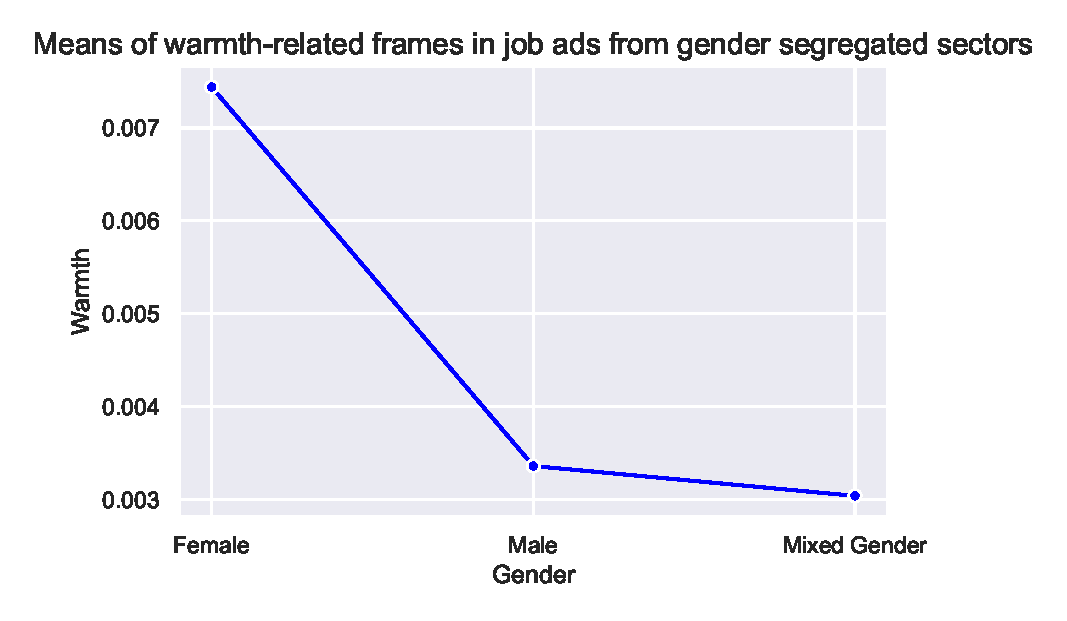
\includegraphics[width=\textwidth]{FT/Figure1.eps}
    \end{center}
    \caption{\textit{Means of the presence of warmth-related frames in job ads from gender-segregated sectors.}}
    \label{figure1}
    \end{figure*}

The second ANOVA model described in the \nameref{analysis} section showed a significant but negligible difference exists in the extent to which competence-related frames are present in job advertisements derived from gender homogeneous and heterogeneous sectors; \textit{F}(2,5700.49)=63.06, \textit{p}=.000, \textit{$\eta^2$}=.004. Hypotheses H2a states that job ads from male-dominated sectors will contain significantly more competence-related frames compared to ads from female-dominated sectors. Post-hoc analysis results were significant. Job ads from male-dominated sectors (\textit{M}=0.584, \textit{SD}=0.357) contained more competence-related frames compared to ads from female-dominated sectors (\textit{M}=0.507, \textit{SD}=0.235), and the effect size was small to medium; \textit{M}\textsubscript{differernce}=.077, \textit{SE}=.007, \textit{p}=.001, \textit{$\eta^2$}=.021. Thus, H2a is also supported.

\begin{table}[ht]
    \small\sf\centering
    \caption{\textit{Games-Howell post-hoc comparisons for gender-segregated sectors and competence-related frames}}
    \label{table6}
    \vskip 4pt
    \resizebox{\linewidth}{!}{%
    \begin{threeparttable}
    \begin{tabular}[]{@{}lccccccccc@{}}
    \toprule
    \multicolumn{10}{c}{Dependent Variable: Competence-Related Frames}\\
    \midrule
    \multicolumn{2}{c}{Sector Comparison} & \multirow{2}{*}{\makecell[c]{\textit{Mean}\\\textit{Difference}}} & \multicolumn{2}{c}{95\% CI} & \multirow{2}{*}{\textit{SE}} & \multirow{2}{*}{\textit{t}} & \multirow{2}{*}{\textit{df}} & \multirow{2}{*}{\textit{p\textsubscript{tukey}}} & \multirow{2}{*}{\textit{$\eta^2$}}\\
    \cmidrule(lr){1-2} \cmidrule(lr){4-5}
    Group 1 & Group 2 & & \textit{LL} & \textit{UL} & & & &\\
    \midrule
    \makecell[l]{Male-\\dominated} & \makecell[l]{Female-\\dominated} & 0.077 & 0.094 & 0.060 & 0.007 & 10.661 & 3815.079 & 0.000*** & 0.021\\
    \makecell[l]{Male-\\dominated} & Mixed-gender & 0.007 & -0.009 & 0.022 & 0.007 & 0.999 & 12080.656 & 0.577 & 0.000\\
    \makecell[l]{Female-\\dominated} & Mixed-gender & -0.071 & -0.089 & -0.053 & 0.008 & -9.218 & 4434.228 & 0.000*** & 0.016\\
    \bottomrule
    \end{tabular}%\\[10pt]
    \begin{tablenotes}
    \footnotesize
    \item * \textit{p} \textless\ .05. ** \textit{p} \textless\ .01. *** \textit{p} \textless\ .001.
    \end{tablenotes}
    \end{threeparttable}
    }
    \end{table}

In the same vein, hypothesis H2b states that job ads from male-dominated sectors will contain significantly more competence-related frames compared to ads from mixed-gender sectors. There was no statistically significant difference in the presence competence-related frames between job ads from male-dominated sectors (\textit{M}=0.584, \textit{SD}=0.357) and ads from mixed-gender sectors (\textit{M}=0.577, \textit{SD}=0.389); \textit{M}\textsubscript{differernce}=.007, \textit{SE}=.007, \textit{p}=.572, \textit{$\eta^2$}=.000. Thus, H2b is rejected.

\begin{figure*}[ht]
    \setlength{\fboxsep}{0pt}%
    \setlength{\fboxrule}{0pt}%
    \begin{center}
    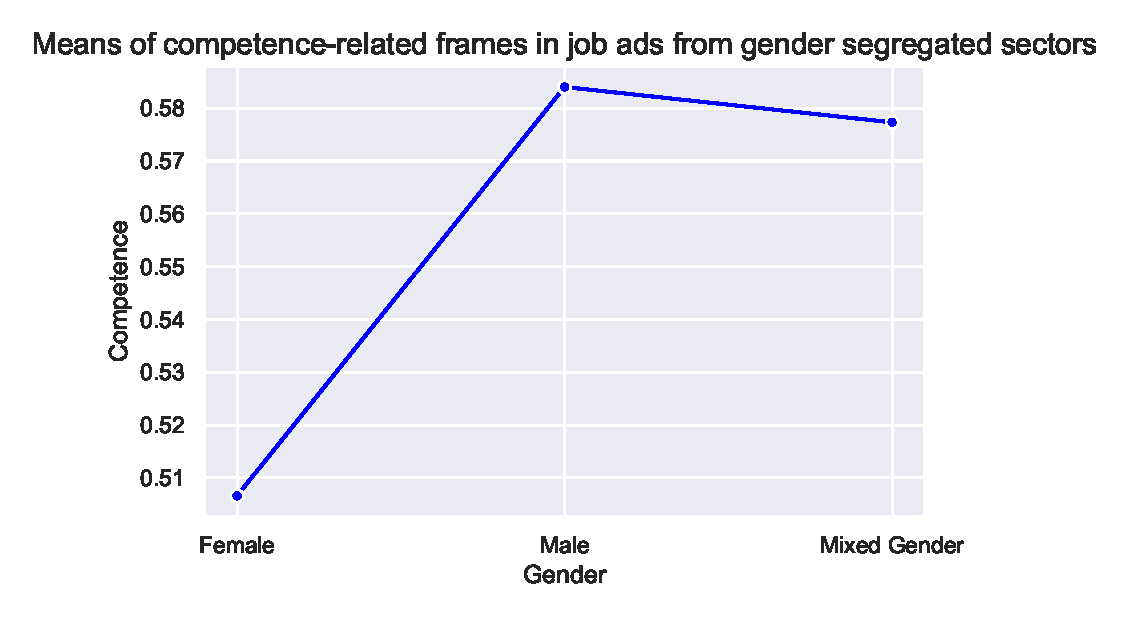
\includegraphics[width=\textwidth]{FT/Figure2.eps}
    \end{center}
    \caption{\textit{Means of the presence of competence-related frames in job ads from gender-segregated sectors.}}
    \label{figure2}
    \end{figure*}

We now turn to the hypotheses examining the relationship between sectoral age segregation and the presence of stereotypical frames in job advertisements. The third ANOVA model described in the Analysis section did not reach statistical significance; \textit{F}(2, 2998.87)=1.79, \textit{p}=.166, \textit{$\eta^2$}=.000. Hypotheses H3a state that job ads from older-dominated sectors will contain significantly more warmth-related frames compared to ads from younger-dominated sectors. This hypothesis was not supported in post-hoc. There was no statistically significant difference in the presence of warmth-related frames between job ads from older-dominated sectors (\textit{M}=0.004, \textit{SD}=0.019) and those from younger-dominated sectors (\textit{M}=0.003, \textit{SD}=0.017); \textit{M}\textsubscript{differernce}=.001, \textit{SE}=.001, \textit{p}=.211, \textit{$\eta^2$}=.001. Thus, H3a is rejected.

\begin{table}[ht]
    \small\sf\centering
    \caption{\textit{Games-Howell post-hoc comparisons for age-segregated sectors and warmth-related frames}}
    \label{table7}
    \vskip 4pt
    \resizebox{\linewidth}{!}{%
    \begin{threeparttable}
    \begin{tabular}[]{@{}lccccccccc@{}}
    \toprule
    \multicolumn{10}{c}{Dependent Variable: Warmth-Related Frames}\\
    \midrule
    \multicolumn{2}{c}{Sector Comparison} & \multirow{2}{*}{\makecell[c]{\textit{Mean}\\\textit{Difference}}} & \multicolumn{2}{c}{95\% CI} & \multirow{2}{*}{\textit{SE}} & \multirow{2}{*}{\textit{t}} & \multirow{2}{*}{\textit{df}} & \multirow{2}{*}{\textit{p\textsubscript{tukey}}} & \multirow{2}{*}{\textit{$\eta^2$}}\\
    \cmidrule(lr){1-2} \cmidrule(lr){4-5}
    Group 1 & Group 2 & & \textit{LL} & \textit{UL} & & & &\\
    \midrule
    \makecell[l]{Older-\\dominated} & \makecell[l]{Younger -\\dominated} & 0.000 & 0.000 & 0.002 & 0.000 & 1.686 & 2444.017 & 0.211 & 0.001\\
    \makecell[l]{Older-\\dominated} & Mixed-age & 0.000 & 0.001 & 0.000 & 0.000 & 1.600 & 5122.627 & 0.246 & 0.000\\
    \makecell[l]{Younger -\\dominated} & Mixed-age & 0.000 & 0.000 & 0.002 & 0.000 & -0.740 & 1550.435 & 0.721 & 0.000\\
    \bottomrule
    \end{tabular}%\\[10pt]
    \begin{tablenotes}
    \footnotesize
    \item * \textit{p} \textless\ .05. ** \textit{p} \textless\ .01. *** \textit{p} \textless\ .001.
    \end{tablenotes}
    \end{threeparttable}
    }
    \end{table}

Hypothesis H3b investigates a similar premise and states that job advertisements from older-dominated sectors will contain significantly more warmth-related frames compared to job advertisements from mixed-age sectors. Post-hoc results were not significant. There was no statistically significant difference in the presence of warmth-related frames between job ads from older-dominated sectors (\textit{M}=0.004, \textit{SD}=0.019) and those from mixed-age sectors (\textit{M}=0.004, \textit{SD}=0.017); \textit{M}\textsubscript{differernce}=.001, \textit{SE}=.000, \textit{p}=.246, \textit{$\eta^2$}=.000. Thus, H3b is also rejected.

\begin{figure*}[ht]
    \setlength{\fboxsep}{0pt}%
    \setlength{\fboxrule}{0pt}%
    \begin{center}
    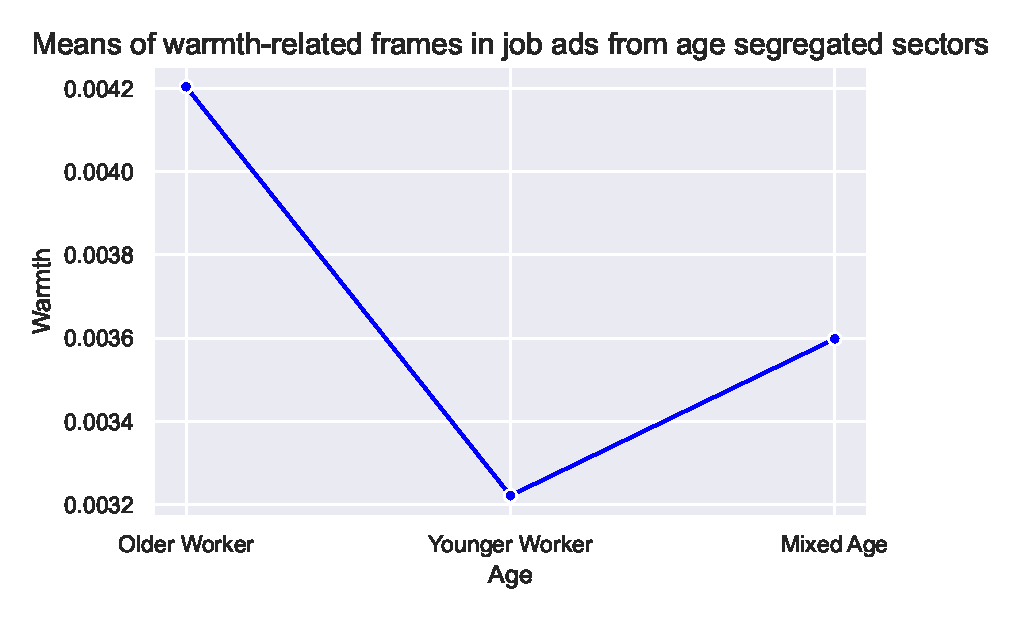
\includegraphics[width=\textwidth]{FT/Figure3.eps}
    \end{center}
    \caption{\textit{Means of the presence of warmth-related frames in job ads from age-segregated sectors.}}
    \label{figure3}
    \end{figure*}

The last ANOVA model described in the Analysis section detected a significant but negligible difference at \textit{F}(2, 2979.12)=36.06, \textit{p}=.000, \textit{$\eta^2$}=.006. Hypothesis H4a states that job ads from younger-dominated sectors will contain significantly more competence-related frames compared to ads from older-dominated sectors. Post-hoc analysis results were significant. Job ads from younger-dominated sectors (\textit{M}=0.644, \textit{SD}=0.399) contained significantly more competence-related frames compared to ads from older-dominated sectors (\textit{M}=0.593, \textit{SD}=0.356), however, the effect size was negligible; \textit{M}\textsubscript{differernce}=.051, \textit{SE}=.013, \textit{p}=.001, \textit{$\eta^2$}=.004. Thus, H4a is supported, however, results should be interpreted with caution.

\begin{table}[ht]
    \small\sf\centering
    \caption{\textit{Games-Howell post-hoc comparisons for age-segregated sectors and competence-related frames}}
    \label{table8}
    \vskip 4pt
    \resizebox{\linewidth}{!}{%
    \begin{threeparttable}
    \begin{tabular}[]{@{}lccccccccc@{}}
    \toprule
    \multicolumn{10}{c}{Dependent Variable: Competence-Related Frames}\\
    \midrule
    \multicolumn{2}{c}{Sector Comparison} & \multirow{2}{*}{\makecell[c]{\textit{Mean}\\\textit{Difference}}} & \multicolumn{2}{c}{95\% CI} & \multirow{2}{*}{\textit{SE}} & \multirow{2}{*}{\textit{t}} & \multirow{2}{*}{\textit{df}} & \multirow{2}{*}{\textit{p\textsubscript{tukey}}} & \multirow{2}{*}{\textit{$\eta^2$}}\\
    \cmidrule(lr){1-2} \cmidrule(lr){4-5}
    Group 1 & Group 2 & & \textit{LL} & \textit{UL} & & & &\\
    \midrule
    \makecell[l]{Younger -\\dominated} & \makecell[l]{Older-\\dominated} & 0.051 & 0.082 & 0.021 & 0.013 & 3.939 & 2020.063 & 0.000*** & 0.004\\
    \makecell[l]{Younger -\\dominated} & Mixed-age & 0.089 & 0.117 & 0.061 & 0.012 & 7.428 & 1487.541 & 0.000*** & 0.012\\
    \makecell[l]{Older-\\dominated} & Mixed-age & 0.037 & 0.054 & 0.021 & 0.007 & 5.186 & 5516.377 & 0.000*** & 0.003\\
    \bottomrule
    \end{tabular}%\\[10pt]
    \begin{tablenotes}
    \footnotesize
    \item * \textit{p} \textless\ .05. ** \textit{p} \textless\ .01. *** \textit{p} \textless\ .001.
    \end{tablenotes}
    \end{threeparttable}
    }
    \end{table}

Hypothesis H4b likewise states that job ads from younger-dominated sectors will contain significantly more competence-related frames compared to ads from mixed-age sectors. Post-hoc analysis results were significant. Job ads from younger-dominated sectors (\textit{M}=0.644, \textit{SD}=0.399) contained significantly more competence-related frames compared to ads from mixed-age sectors (\textit{M}=0.556, \textit{SD}=0.354), and the effect size was small; \textit{M}\textsubscript{differernce}=.089, \textit{SE}=.012, \textit{p}=.001, \textit{$\eta^2$}=.012. Thus, H4b is also supported.

\begin{figure*}[ht]
    \setlength{\fboxsep}{0pt}%
    \setlength{\fboxrule}{0pt}%
    \begin{center}
    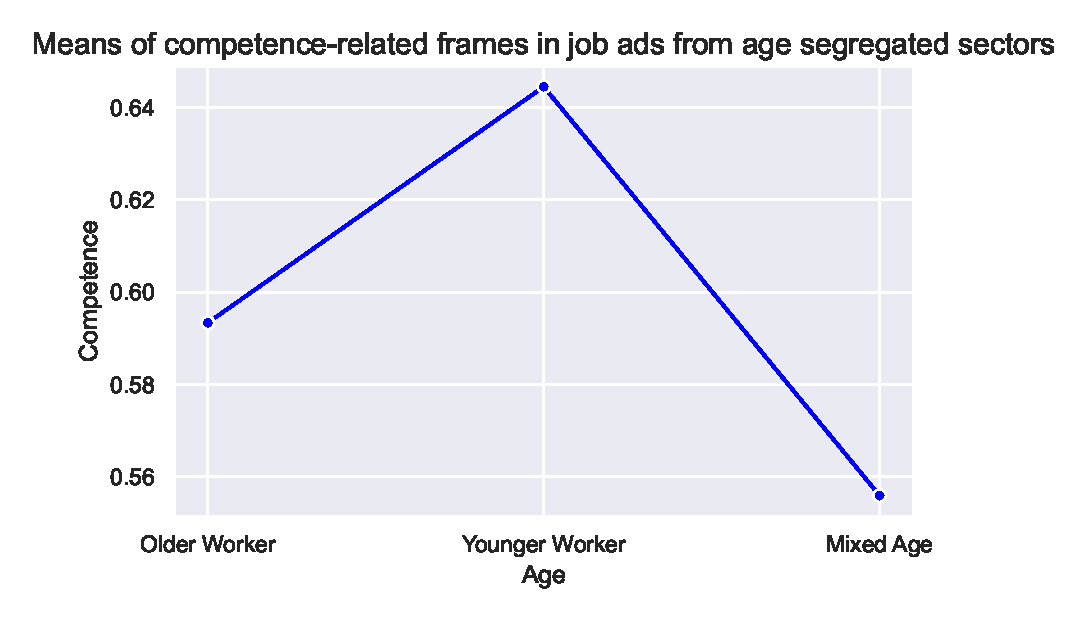
\includegraphics[width=\textwidth]{FT/Figure4.eps}
    \end{center}
    \caption{\textit{Means of the presence of competence-related frames in job ads from age-segregated sectors.}}
    \label{figure4}
    \end{figure*}

\clearpage
\section{Discussion\label{discussion}}
In conducting this study, we set out to outline, identify, and examine the stereotypical frames present in job advertisements as indicated by the differential emphasis on warmth and competence characteristics, and to empirically investigate the link between the presence of such frames and sectoral gender and age segregation. We put forth an operationalization of broad-level gender- and age-related stereotypical frames that is compatible with the axioms of the SCM and adapted specifically to examine early candidate sourcing communication. As per the operationalization presented, the concept of warmth in the occupational domain is communicated by emphasizing an orientation towards people, team and community building, and strong interpersonal characteristics. Conversely, the concept of occupational competence is conveyed by emphasizing productivity, performance on tasks, measurable outcomes, and the display of technical acumen.

With regards to the correlation between gender-stereotypical job advertisements’ framing and sectoral segregation, our findings show that job ads from female-dominated sectors tend to emphasize warmth but de-emphasize competence. This is indicated by the comparability in the presence of warmth-related frames between ads from male-dominated and mixed-gender sectors but a significant difference in the presence of competence-related frames between the female-dominated and mixed-gender sectors (see Figure~\ref{figure1} and Figure~\ref{figure2}). Ads from male-dominated and mixed-gender sectors were comparable in the presence of both types of frames, further indicating differences stem chiefly from the framing of ads from female-dominated sectors.

The presence of warmth-related frames in job ads from female-dominated sectors but not in ads from male-dominated and mixed-gender sectors align with social categorization framing. An emphasis on warmth characteristics as well as a de-emphasis on competence characteristics signals social category-based ownership of warmth-dominant sectors and suggests some endorsement of traditional gender essentialism particularly as it pertains to women. However, these findings may also suggest a different kind of gender essentialism, specifically egalitarian gender essentialism suggested by Cotter et al. \citeyear{cotterEndGenderRevolution2011} to explain the gender-equality paradox observed in liberal egalitarian societies.

Horizontal segregation has been particularly resistant to egalitarian policies and Charles and Grusky \citeyear{charlesEgalitarianismGenderInequality2011} attributed this to liberal egalitarianism sanctioning “essentialist presumption that men and women have fundamentally different tastes, skills, and abilities” (p. 945). Egalitarian essentialism is a response to this reproach. It posits that following the 1990’s “have it all” attitudes to female employment, women in egalitarian societies opted to blend feminist equality with an endorsement of the positive aspects of female essentialist and stereotypical roles; what Cotter et al. called the “egalitarian but traditional” perspective.

A stereotypical attribution of warmth to females in society, and by extension in the workplace, could thus be driven by either traditional gender essentialism or egalitarian gender essentialism. These competing paradigms carry distinct implications for candidate sourcing. Driven by traditional gender essentialism, the use of warmth-related frames may point to rigidity in whom employers envision as an ideal candidate, i.e., a female job seeker, and that a candidate who possesses warmth characteristics but does not conform to the gender ideal is less likely to be considered for the position. Driven by egalitarian gender essentialism, the use of warmth-related frames may be viewed as a neutral sourcing practice that does not incorporate the negative connotations of male primacy not supremacy. In this case, utilizing warmth-related frames not only signals a willingness to hire female workers, but also that warmth characteristics are valued in job seekers of any gender.

It must be noted that in any case Charles and Grusky’s \citeyear{cotterEndGenderRevolution2011} criticism of gender essentialist beliefs carries weight; that an endorsement of even the most positive aspects of such beliefs leaves unexamined how these beliefs were formed, why they differ for different gender groups, and what effects they would have. This criticism becomes particularly relevant when considering that our results showed a significant de-emphasis on competence characteristics in job ads from female-dominated sectors.

Endorsement of either kind of gender essentialist beliefs can lead to emphasis on one stereotype content dimension to the exclusion of the other. From the purview of social categorization framing, the message of job ads framed via warmth and competence may still be perceived as emphasizing social category ownership of a sector rather than its openness to individuals who possess the emphasized characteristic. In gender essentialist domains, this reasoning in response to stereotypical frames is especially likely as studies show endorsement of essentialist beliefs predict increased salience of the emphasized category as well as promote stereotyping beyond other commonly researched individual differences \shortcite{bastianPsychologicalEssentialismStereotype2006,leichtCounterStereotypesFeminismPromote2017,paukerRaceSalienceEssentialist2010}. Ultimately, the lopsided use of warmth- and competence-related frames in female-dominated sectors reinforces gender stereotypes pertaining to women regardless of the underlying belief system.

With regards to the correlation between age-stereotypical job advertisements framing and sectoral segregation, our findings show no difference in the presence of warmth-related frames among age homogeneous and heterogeneous sector categories. Conversely, ads from younger dominated sectors were significantly more likely to contain competence-related frames compared to ads from older dominated sectors as well as mixed-age sectors. Job ads from older-dominated sectors also contained significantly more competence-related frames compared to mixed-age sectors.

These results are in line with studies that indicate warmth primacy is not as readily transferable to the context of hiring and recruitment despite older workers being stereotyped as warm. Findings from Abrams et al. \citeyear{abramsOldUnemployableHow2016} and Krings et al. \citeyear{kringsStereotypicalInferencesMediators2011} show that warmth characteristics are consistently linked to older workers, however, a requirement of warmth characteristics in an offered position did not predict a preference for older job seekers. Furthermore, Krings et al. \citeyear{kringsStereotypicalInferencesMediators2011} found that when explicitly evaluating candidates for hiring as opposed to a context-free evaluation, older job seekers were perceived as less warm than their younger counterparts.

A likely explanation for this disparity is that for older workers, workplace-related negative competence stereotypes as opposed to positive warmth stereotypes are more robust and salient when employers are explicitly considering productivity goals. Indeed, studies point to this being the case as employers consistently rate older workers lower on productivity \shortcite{kroonReliableUnproductiveStereotypes2018,vandalenProductivityOlderWorkers2010}. Nevertheless, our findings on the presence of warmth-related frames in job ads from female-dominated sectors suggest more research is needed to explain this disparity between gender-based and age-based warmth stereotypes. Researchers may benefit from exploring confounding factors such as differences in value ascribed to warmth characteristics during hiring, valence of stereotype content \shortcite{suitnerRoleValencePerception2008}, or perceptions of older workers in a given context \shortcite{hennekamEmployabilityOlderWorkers2015}.

\subsection{Societal Implications\label{societal_implications}}
Tentatively, all findings presented indicate partial support for social categorization framing in candidate sourcing and its exercise in employer communication addressing different gender and age groups. Although we advise caution in drawing clear-cut conclusions regarding the extent to which stereotypical frames are present in job advertisements due to the small effect sizes achieved, the significant results point to the merit of our investigation. The differences in warmth- and competence-related frames mostly in favor of homogeneous sectors indicate an emphasis on stereotypical gender and age characteristics in these sectors that is not readily apparent but is nonetheless present.

These results could prove consequential in the context of automated candidate sourcing as more HR processes move to online spaces. Online job search platforms have recently begun developing and deploying various content-based recommender systems (CBR). The predictive algorithms behind these e-Recruitment tools leverage textual features of job advertisements in order to target job seekers \shortcite{pejic-bachTextMiningIndustry2020,shiSalienceMarketawareSkill2020}. With the current advancements in natural language processing, the novel implementations of CBR systems are able to detect subtle textual indicators of bias and inadvertently perpetuate inequitable candidate sourcing \shortcite{singhalUseDeepLearning2017}. Amazon, for instance, discontinued its machine learning-based recruitment tool after the algorithms learned to downgrade or even exclude resumes that contained terms like ‘women’s chess club’ or names of all-women’s colleges \shortcite{dastinAmazonScrapsSecret2018}. Although this example may be an excess within the larger context of automated hiring and recruitment, it does show the potential impact of these approaches if not addressed. The results of this study thus provide empirical foundation for examining stereotypical frames in job ads as automation becomes the norm in candidate sourcing.

Beyond consequences for candidate sourcing, the presence of stereotypical frames in early employer communication has consequences for job seekers who are exposed to these messages. According to Yang \citeyear{Yang2015a}, the significant emphasis on dominant social category characteristics serves to makes salient the self-to-others social distance, consequently activating social category stereotyping directed towards outgroups members as well as the self \shortcite{Steele1997}. Particular to employer communication, studies indicate usage of such communication, although may initially help target sourcing efforts, ultimately narrows the pool of job seekers who feel addressed by employers’ communication and feel appealed to apply \shortcite{zhuUnderstandingRoleOrganizational2021}. Exposure to such communication can have substantial consequences for potential candidates’ perceived social belonging, stereotype threat perceptions, and the level of trust candidates have towards professional settings \shortcite{purdie-vaughnsSocialIdentityContingencies2008,waltonQuestionBelongingRace2007}. Emphasis on stereotypical aspects of a position can also lead job seekers to self-select or self-eliminate based on perceived role incongruity, further narrowing the pool of potential candidates and ultimately decreasing workplace diversity \shortcite{henningsenWhereAreWomen2021}.

\subsection{Limitations and Recommendations\label{limitations_and_recommendations}}
As with any endeavor, this study has some limitations of note. The differences in job ad framing, although exhibiting small effect sizes, are meaningful in the context of the larger media studies paradigm \shortcite{Perloff2013}. Nonetheless, we advise caution in interpreting the results particularly given the imbalanced class distribution in our training and annotated dataset. We attempted to mitigate the imbalance by implementing cost-sensitive learning, removing outliers, and employing tests that accounted violated assumptions of normality, however, such distributions are an empirical reality of using online data. To address this, future researchers may benefit from applying predefined quotas when sampling.

Limitations also arose with regards to the structure of job advertisements. We noted that job ads follow a set format. For the ads we examined, warmth-related sentences are more likely to appear at the opening and conclusion of a job ad and competence-related sentences are likely to appear in the middle. We also observed that the middle sections are customarily where job requirements and tasks are stated, thus may prove relevant to examining message framing. We attempted to mitigate both issues discussed thus far by including exploratory variables indicating the framing of sentences specifically related to job tasks and requirements, however, reliability of those variables proved low and we did not include them in analysis. We find that a formalization of job advertisements’ formats may be necessary to furthering organizational communication framing studies as measures relying on sentences and task mentions only provide a partial picture.

With regards to the usage of concepts related to warmth and competence in job advertisements, we find that some qualities cannot be neatly categorized as fitting into one dimension or the other. For instance, concepts related to global or multicultural organizational aspects had to be singled out and described separately in our operationalization (see Codebook). On one hand, emphasis on these aspects could convey an inclusive and diverse workplace, which coders perceived as emphasizing warmth. On the other, many job ads used these aspects to indicate global market presence, which to coders highlighted an organization’s competence. In line with many items we encountered, emphasizing an organization’s multiculturalism seemed to serve both purposes simultaneously, consequently the concept could not be categorized as definitively as preferred. Future researchers are invited to explore offshoots of the SCM, for example, the SCM facet model Agency-Communion-Inventory \shortcite(AC-IN; ){abeleFacetsFundamentalContent2016}, which distinguish dimensions through motivations, abilities, and similar cognitive mechanisms. We contend that approaching warmth and competence dimensions through their underlying drivers may help delineate concepts in text and constrain their operationalization to factors pertinent to the topic under study.

\subsection{Conclusion\label{conclusion}}
Summarily, the study at hand invites a thoughtful examination of inequitable hiring practices at the sourcing phase. We offer an operationalization of social categorization frames in candidate sourcing communication based on the stereotype content model’s dimensions of warmth and competence. The framing of job ads from gender and age-segregated sectors partially aligned with stereotypical attribution of these characteristics to the respective gender and age groups, however, our results also point to complex contextual factors at play. Our findings offer researchers a framework for investigating variations in stereotypically framed employer communication as a function of variations in social category-based sectoral segregation. We also provide industry professionals with insight into the interplay between the status quo of their job domains, whether and how it is reflected in employer communication, and the manner in which job advertisements from such domains may be perceived by job seekers from different gender and age groups. Our work thus invites a more rigorous assessment of HR sourcing practices and offers a roadmap for diversity-minded employers to address bias hiring at its genesis.

\theendnotes

\bibliography{Bias_in_Candidate_Sourcing.bib}

\clearpage
\newpage
\section{Appendix A\label{appendix_a}}

\begin{landscape}
    \begin{longtabu}{>{\hspace{0pt}}m{0.167\linewidth}>{\hspace{0pt}}m{0.104\linewidth}>{\centering\hspace{0pt}}m{0.056\linewidth}>{\centering\hspace{0pt}}m{0.104\linewidth}>{\centering\hspace{0pt}}m{0.054\linewidth}>{\centering\hspace{0pt}}m{0.104\linewidth}>{\centering\hspace{0pt}}m{0.056\linewidth}>{\centering\hspace{0pt}}m{0.102\linewidth}>{\centering\hspace{0pt}}m{0.056\linewidth}>{\centering\hspace{0pt}}m{0.048\linewidth}>{\centering\arraybackslash\hspace{0pt}}m{0.075\linewidth}}
    \caption{\textit{Sectoral Age and Gender Composition and Segregation}}
    \label{table9}
    \hline
    \multicolumn{11}{>{\centering\arraybackslash\hspace{0pt}}m{0.926\linewidth}}{Jobs Count per Sector (x 1000)} \\*
    \multicolumn{1}{>{\Centering\hspace{0pt}}m{0.167\linewidth}}{\multirow{3}{0.167\linewidth}{\hspace{0pt}\Centering{}Industry   class / branch (SIC2008)}} & \multicolumn{4}{>{\Centering\hspace{0pt}}m{0.318\linewidth}}{Gender} & \multicolumn{4}{>{\Centering\hspace{0pt}}m{0.318\linewidth}}{Age} & \multicolumn{2}{>{\Centering\hspace{0pt}}m{0.123\linewidth}}{\multirow{2}{0.123\linewidth}{\hspace{0pt}\Centering{}Total   Employment}} \\*
    \cline{2-9}
    \multicolumn{1}{>{\Centering\hspace{0pt}}m{0.167\linewidth}}{} & \multicolumn{2}{>{\Centering\hspace{0pt}}m{0.16\linewidth}}{Female} & \multicolumn{2}{>{\Centering\hspace{0pt}}m{0.158\linewidth}}{Male} & \multicolumn{2}{>{\Centering\hspace{0pt}}m{0.16\linewidth}}{Older (= 45)} & \multicolumn{2}{>{\Centering\hspace{0pt}}m{0.158\linewidth}}{Younger ( 45)} & \multicolumn{2}{>{\Centering\hspace{0pt}}m{0.123\linewidth}}{} \\*
    \cline{2-11}
    \multicolumn{1}{>{\Centering\hspace{0pt}}m{0.167\linewidth}}{} & \textit{n} & \% & \textit{n} & \% & \textit{n} & \% & \textit{n} & \% & \textit{n} & Total \% \endfirsthead
    \hline
    AU All economic activities & 4030 &  & 4363 &  & 3497 &  & 4895 &  & 8392 &  \\
    AF Agriculture and industry & 270 & \uline{21\%} & 1015 & \textbf{79\%} & 650 & 51\% & 635 & 49\% & 1286 & 5.09\% \\
    A  Agriculture, forestry and fishing & 39 & 35\% & 73 & 65\% & 40 & 36\% & 71 & 63\% & 112 & 0.44\% \\
    BF Manifacturing and energy & 232 & \uline{20\%} & 942 & \textbf{80\%} & 611 & 52\% & 564 & 48\% & 1174 & 4.65\% \\
    BE Industry (no construction), energy & 190 & \uline{23\%} & 649 & \textbf{77\%} & 451 & \textbf{54\%} & 386 & 46\% & 839 & 3.32\% \\
    B  Mining and quarrying & 1 & \uline{13\%} & 7 & \textbf{88\%} & 4 & 50\% & 4 & 50\% & 8 & 0.03\% \\
    C  Manufacturing & 174 & \uline{23\%} & 592 & \textbf{77\%} & 413 & \textbf{54\%} & 354 & 46\% & 766 & 3.03\% \\
    D  Energy supply & 7 & \uline{25\%} & 21 & \textbf{75\%} & 15 & \textbf{54\%} & 13 & 46\% & 28 & 0.11\% \\
    E  Water supply and waste management & 7 & \uline{19\%} & 29 & \textbf{81\%} & 21 & \textbf{58\%} & 16 & 44\% & 36 & 0.14\% \\
    F  Construction & 42 & \uline{13\%} & 293 & \textbf{87\%} & 159 & 47\% & 175 & 52\% & 335 & 1.33\% \\
    GN Commercial services & 1813 & 42\% & 2519 & 58\% & 1525 & 35\% & 2807 & 65\% & 4332 & 17.14\% \\
    GI Trade, transport, hotels, catering & 953 & 43\% & 1239 & 57\% & 729 & 33\% & 1463 & 67\% & 2192 & 8.67\% \\
    G  Wholesale and retail trade & 658 & 47\% & 753 & 53\% & 448 & \uline{32\%} & 963 & \textbf{68\%} & 1411 & 5.58\% \\
    H  Transportation and storage & 95 & \uline{25\%} & 290 & \textbf{75\%} & 205 & \textbf{53\%} & 181 & 47\% & 386 & 1.53\% \\
    I  Accommodation and food serving & 199 & 50\% & 196 & 50\% & 75 & \uline{19\%} & 320 & \textbf{81\%} & 395 & 1.56\% \\
    J  Information and communication & 80 & 28\% & 209 & 72\% & 95 & 33\% & 195 & 67\% & 289 & 1.14\% \\
    K  Financial institutions & 107 & 39\% & 165 & 61\% & 145 & \textbf{53\%} & 128 & 47\% & 272 & 1.08\% \\
    L  Renting, buying, selling real estate & 33 & 49\% & 35 & 51\% & 36 & \textbf{53\%} & 33 & 49\% & 68 & 0.27\% \\
    MN Business services & 639 & 42\% & 871 & 58\% & 521 & 35\% & 989 & 65\% & 1510 & 5.97\% \\
    M  Other specialized business services & 220 & 42\% & 309 & 58\% & 206 & 39\% & 322 & 61\% & 529 & 2.09\% \\
    N  Renting and other business support & 419 & 43\% & 562 & 57\% & 314 & \uline{32\%} & 668 & \textbf{68\%} & 981 & 3.88\% \\
    OU Noncommercial services & 1947 & \textbf{70\%} & 828 & 30\% & 1324 & 48\% & 1451 & 52\% & 2775 & 10.98\% \\
    OQ Government and care & 1790 & \textbf{71\%} & 720 & 29\% & 1217 & 48\% & 1292 & 51\% & 2510 & 9.93\% \\
    O  Public administration and services & 230 & 43\% & 307 & 57\% & 303 & \textbf{56\%} & 234 & 44\% & 537 & 2.12\% \\
    P  Education & 353 & 65\% & 189 & 35\% & 253 & 47\% & 287 & 53\% & 541 & 2.14\% \\
    Q  Health and social work activities & 1208 & \textbf{84\%} & 224 & 16\% & 660 & 46\% & 770 & 54\% & 1432 & 5.67\% \\
    RU Culture, recreation, other services & 156 & 59\% & 108 & 41\% & 106 & 40\% & 158 & 60\% & 264 & 1.04\% \\
    R  Culture, sports and recreation & 70 & 53\% & 63 & 48\% & 49 & 37\% & 83 & 63\% & 132 & 0.52\% \\
    S  Other service activities & 87 & 66\% & 45 & 34\% & 55 & 42\% & 75 & 57\% & 132 & 0.52\% \\ \hline
    \hline
    Total   (excluding AU) & 12019 (47.56\%) &  & 13253 (52.44\%) &  & 14127 (42.06\%) &  & 19532 (57.92\%) &  & 25272 & 100.00\% \\
    \hline
    Source: CBS &  & \multicolumn{1}{>{\hspace{0pt}}m{0.056\linewidth}}{} & \multicolumn{1}{>{\hspace{0pt}}m{0.104\linewidth}}{} & \multicolumn{1}{>{\hspace{0pt}}m{0.054\linewidth}}{} & \multicolumn{1}{>{\hspace{0pt}}m{0.104\linewidth}}{} & \multicolumn{1}{>{\hspace{0pt}}m{0.056\linewidth}}{} & \multicolumn{1}{>{\hspace{0pt}}m{0.102\linewidth}}{} & \multicolumn{1}{>{\hspace{0pt}}m{0.056\linewidth}}{} & \multicolumn{1}{>{\hspace{0pt}}m{0.048\linewidth}}{} & \multicolumn{1}{>{\hspace{0pt}}m{0.075\linewidth}}{} \\
    \multicolumn{11}{>{\hspace{0pt}}m{0.926\linewidth}}{\textit{Note.} \textbf{Bolded percentages} indicate sectors that are segregated.\par{} Threshold for gender = 47.56\% ± 20\%\par{} Threshold for age = 42.06\% ± 10\%}\\
    \end{longtabu}
    \end{landscape}

\begin{figure*}[ht]
\setlength{\fboxsep}{0pt}%
\setlength{\fboxrule}{0pt}%
\begin{center}
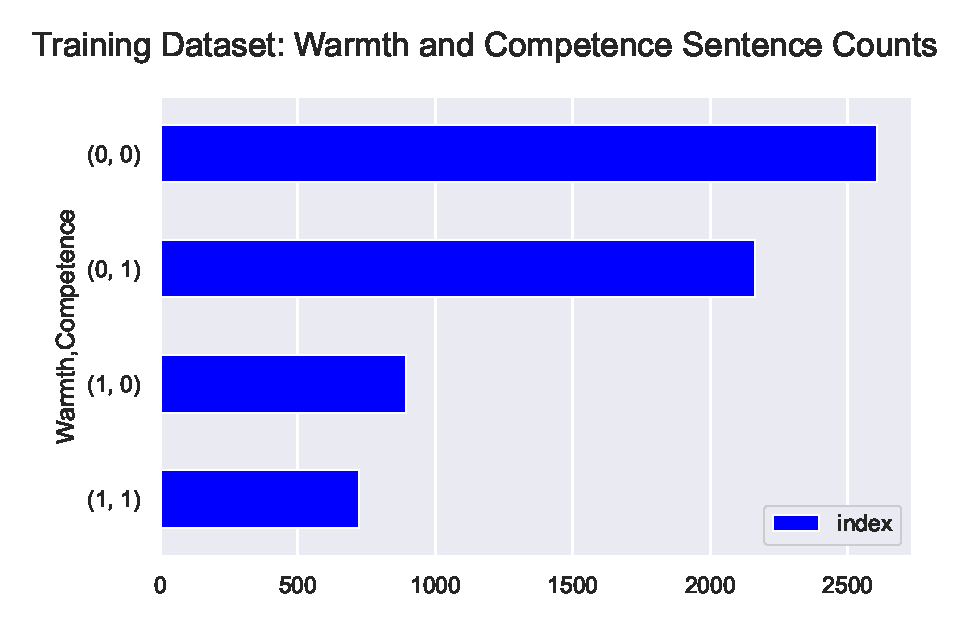
\includegraphics[width=0.90\textwidth]{FT/Figure5.eps}
\end{center}
\caption{\textit{Means of the presence of warmth-related frames in job ads from age-segregated sectors.}}
\label{figure5}
\end{figure*}

\begin{landscape}
    \begin{longtable}[l]{lcccccccc}
    \caption{Model evaluation scores for warmth-related frames classifiers}
    \label{table10}
    \hline
    & \multicolumn{8}{c}{Warmth} \\ \hline
    \endhead
    %
    \multirow{2}{*}{Classifiers} & \multicolumn{8}{c}{Count Vectorizer} \\ \cline{2-9}
    & Mean   Validation Score & Accuracy & Precision & Recall & F1-score & ROC & AUC & Loss \\ \hline
    Dummy Classifier - Most   Frequent & 0.74 & 0.74 & 0.00 & 0.00 & 0.00 & 0.50 & 0.50 & 8.90 \\
    Dummy Classifier - Stratified & 0.62 & 0.62 & 0.26 & 0.25 & 0.25 & 0.50 & 0.50 & 13.12 \\
    Multinomial Naive Bayes & 0.80 & 0.82 & 0.68 & 0.59 & 0.63 & 0.75 & 0.80 & 0.71 \\
    K-Nearest Neighbors & 0.78 & 0.79 & 0.67 & 0.36 & 0.47 & 0.65 & 0.74 & 3.43 \\
    Logistic Regression & 0.82 & 0.83 & 0.68 & 0.67 & 0.67 & 0.78 & 0.86 & 0.43 \\
    Passive Aggressive Classifier & 0.80 & 0.81 & 0.64 & 0.60 & 0.62 & - & - & - \\
    Linear Support Vector Machine & 0.80 & 0.81 & 0.63 & 0.63 & 0.63 & - & - & - \\
    Decision Tree & 0.74 & 0.80 & 0.60 & 0.61 & 0.61 & 0.74 & 0.74 & 6.92 \\
    Random Forest & 0.79 & 0.83 & 0.75 & 0.50 & 0.60 & 0.72 & 0.89 & 0.42 \\
    Extra Trees Classifier & 0.80 & 0.84 & 0.76 & 0.53 & 0.62 & 0.73 & 0.87 & 0.98 \\
    Gradient Boosting Machine & 0.78 & 0.80 & 0.67 & 0.49 & 0.56 & 0.70 & 0.82 & 0.63 \\
    Adaptive Boosting Machine & 0.78 & 0.81 & 0.71 & 0.47 & 0.56 & 0.70 & 0.82 & 0.68 \\
    Stacking Classifier & 0.80 & 0.82 & 0.71 & 0.55 & 0.62 & 0.73 & 0.87 & 0.56 \\
    Voting Classifier & 0.82 & 0.84 & 0.74 & 0.60 & 0.66 & 0.76 & 0.88 & 0.37 \\ \hline
    \multirow{2}{*}{Classifiers} & \multicolumn{8}{c}{TF-IDF Vectorizer} \\ \cline{2-9}
    & Mean   Validation Score & Accuracy & Precision & Recall & F1-score & ROC & AUC & Loss \\ \hline
    Dummy Classifier - Most   Frequent & 0.74 & 0.74 & 0.00 & 0.00 & 0.00 & 0.50 & 0.50 & 8.90 \\
    Dummy Classifier - Stratified & 0.62 & 0.62 & 0.26 & 0.25 & 0.25 & 0.50 & 0.50 & 13.12 \\
    Multinomial Naive Bayes & 0.75 & 0.78 & 0.79 & 0.19 & 0.31 & 0.59 & 0.80 & 0.47 \\
    K-Nearest Neighbors & 0.77 & 0.78 & 0.64 & 0.34 & 0.44 & 0.64 & 0.73 & 3.36 \\
    \textbf{Logistic Regression} & \textbf{0.80} & \textbf{0.81} & \textbf{0.61} & \textbf{0.74} & \textbf{0.67} & \textbf{0.79} & \textbf{0.87} & \textbf{0.47} \\
    Passive Aggressive Classifier & 0.79 & 0.81 & 0.63 & 0.63 & 0.63 & - & - & - \\
    Linear Support Vector Machine & 0.80 & 0.83 & 0.65 & 0.72 & 0.68 & - & - & - \\
    Decision Tree & 0.74 & 0.78 & 0.57 & 0.65 & 0.61 & 0.74 & 0.74 & 7.31 \\
    Random Forest & 0.79 & 0.83 & 0.75 & 0.52 & 0.62 & 0.73 & 0.89 & 0.38 \\
    Extra Trees Classifier & 0.80 & 0.83 & 0.76 & 0.51 & 0.61 & 0.73 & 0.87 & 0.94 \\
    Gradient Boosting Machine & 0.77 & 0.80 & 0.64 & 0.55 & 0.59 & 0.72 & 0.83 & 0.86 \\
    Adaptive Boosting Machine & 0.77 & 0.81 & 0.67 & 0.50 & 0.57 & 0.71 & 0.82 & 0.68 \\
    Stacking Classifier & 0.80 & 0.84 & 0.71 & 0.62 & 0.66 & 0.77 & 0.88 & 0.50 \\
    Voting Classifier & 0.79 & 0.84 & 0.80 & 0.49 & 0.61 & 0.72 & 0.89 & 0.39 \\ \hline
    \multirow{2}{*}{Classifiers} & \multicolumn{8}{c}{Feature Union} \\ \cline{2-9}
    & Mean   Validation Score & Accuracy & Precision & Recall & F1-score & ROC & AUC & Loss \\ \hline
    Dummy Classifier - Most   Frequent & 0.74 & 0.74 & 0.00 & 0.00 & 0.00 & 0.50 & 0.50 & 8.90 \\
    Dummy Classifier - Stratified & 0.62 & 0.62 & 0.26 & 0.25 & 0.25 & 0.50 & 0.50 & 13.12 \\
    Multinomial Naive Bayes & 0.79 & 0.82 & 0.68 & 0.58 & 0.63 & 0.74 & 0.79 & 0.82 \\
    K-Nearest Neighbors & 0.77 & 0.81 & 0.70 & 0.44 & 0.54 & 0.69 & 0.76 & 3.02 \\
    Logistic Regression & 0.82 & 0.83 & 0.68 & 0.67 & 0.68 & 0.78 & 0.86 & 0.42 \\
    Passive Aggressive Classifier & 0.79 & 0.80 & 0.61 & 0.62 & 0.62 & - & - & - \\
    Linear Support Vector Machine & 0.80 & 0.81 & 0.63 & 0.62 & 0.63 & - & - & - \\
    Decision Tree & 0.75 & 0.79 & 0.58 & 0.66 & 0.62 & 0.75 & 0.75 & 7.20 \\
    Random Forest & 0.80 & 0.84 & 0.76 & 0.54 & 0.63 & 0.74 & 0.89 & 0.37 \\
    Extra Trees Classifier & 0.80 & 0.83 & 0.74 & 0.53 & 0.62 & 0.73 & 0.88 & 0.88 \\
    Gradient Boosting Machine & 0.76 & 0.81 & 0.65 & 0.54 & 0.59 & 0.72 & 0.83 & 0.83 \\
    Adaptive Boosting Machine & 0.77 & 0.81 & 0.67 & 0.50 & 0.57 & 0.71 & 0.82 & 0.68 \\
    Stacking Classifier & 0.80 & 0.83 & 0.73 & 0.57 & 0.64 & 0.75 & 0.88 & 0.50 \\
    Voting Classifier & 0.82 & 0.84 & 0.74 & 0.59 & 0.65 & 0.76 & 0.88 & 0.37 \\ \hline
    \multicolumn{9}{l}{\textit{Note.} \textbf{Bolded scores} indicate final selected model. “-” indicates values that are not calculated by evaluation modules.}
    \end{longtable}
\end{landscape}

\begin{landscape}
    \begin{longtable}[l]{lcccccccc}
    \caption{Model evaluation scores for competence-related frames classifiers}
    \label{table11}
    \hline
    & \multicolumn{8}{c}{Warmth} \\ \hline
    \endhead
    %
    \multirow{2}{*}{Classifiers} & \multicolumn{8}{c}{Count Vectorizer} \\ \cline{2-9}
    & Mean   Validation Score & Accuracy & Precision & Recall & F1-score & ROC & AUC & Loss \\ \hline
    Dummy Classifier - Most   Frequent & 0.57 & 0.57 & 0.00 & 0.00 & 0.00 & 0.50 & 0.50 & 14.89 \\
    Dummy Classifier - Stratified & 0.52 & 0.50 & 0.42 & 0.46 & 0.44 & 0.49 & 0.49 & 17.42 \\
    Multinomial Naive Bayes & 0.73 & 0.78 & 0.70 & 0.85 & 0.77 & 0.79 & 0.85 & 0.78 \\
    K-Nearest Neighbors & 0.68 & 0.71 & 0.74 & 0.49 & 0.59 & 0.68 & 0.75 & 4.14 \\
    Logistic Regression & 0.75 & 0.80 & 0.77 & 0.75 & 0.76 & 0.79 & 0.87 & 0.46 \\
    Passive Aggressive Classifier & 0.73 & 0.77 & 0.74 & 0.73 & 0.73 & - & - & - \\
    Linear Support Vector Machine & 0.74 & 0.78 & 0.76 & 0.73 & 0.75 & - & - & - \\
    Decision Tree & 0.71 & 0.73 & 0.70 & 0.65 & 0.67 & 0.72 & 0.71 & 8.78 \\
    Random Forest & 0.73 & 0.78 & 0.76 & 0.70 & 0.73 & 0.77 & 0.86 & 0.50 \\
    Extra Trees Classifier & 0.74 & 0.78 & 0.77 & 0.70 & 0.74 & 0.77 & 0.87 & 0.87 \\
    Gradient Boosting Machine & 0.71 & 0.75 & 0.75 & 0.63 & 0.68 & 0.73 & 0.82 & 0.59 \\
    Adaptive Boosting Machine & 0.71 & 0.75 & 0.75 & 0.62 & 0.68 & 0.73 & 0.80 & 0.69 \\
    Stacking Classifier & 0.74 & 0.78 & 0.74 & 0.77 & 0.75 & 0.78 & 0.86 & 0.56 \\
    Voting Classifier & 0.77 & 0.81 & 0.76 & 0.81 & 0.79 & 0.81 & 0.88 & 0.43 \\ \hline
    \multirow{2}{*}{Classifiers} & \multicolumn{8}{c}{TF-IDF Vectorizer} \\ \cline{2-9}
    & Mean   Validation Score & Accuracy & Precision & Recall & F1-score & ROC & AUC & Loss \\ \hline
    Dummy Classifier - Most   Frequent & 0.57 & 0.57 & 0.00 & 0.00 & 0.00 & 0.50 & 0.50 & 14.89 \\
    Dummy Classifier - Stratified & 0.52 & 0.50 & 0.42 & 0.46 & 0.44 & 0.49 & 0.49 & 17.42 \\
    Multinomial Naive Bayes & 0.74 & 0.79 & 0.72 & 0.82 & 0.77 & 0.79 & 0.86 & 0.48 \\
    K-Nearest Neighbors & 0.68 & 0.72 & 0.73 & 0.55 & 0.63 & 0.70 & 0.77 & 3.34 \\
    Logistic Regression & 0.74 & 0.79 & 0.72 & 0.82 & 0.77 & 0.79 & 0.86 & 0.49 \\
    Passive Aggressive Classifier & 0.71 & 0.77 & 0.72 & 0.76 & 0.74 & - & - & - \\
    Linear Support Vector Machine & 0.74 & 0.79 & 0.73 & 0.81 & 0.77 & - & - & - \\
    Decision Tree & 0.71 & 0.74 & 0.70 & 0.70 & 0.70 & 0.73 & 0.73 & 8.58 \\
    Random Forest & 0.74 & 0.79 & 0.75 & 0.78 & 0.76 & 0.79 & 0.87 & 0.48 \\
    Extra Trees Classifier & 0.75 & 0.80 & 0.76 & 0.77 & 0.76 & 0.79 & 0.87 & 0.78 \\
    Gradient Boosting Machine & 0.70 & 0.75 & 0.73 & 0.66 & 0.69 & 0.74 & 0.81 & 0.60 \\
    Adaptive Boosting Machine & 0.70 & 0.74 & 0.73 & 0.63 & 0.68 & 0.73 & 0.79 & 0.68 \\
    Stacking Classifier & 0.74 & 0.79 & 0.74 & 0.80 & 0.77 & 0.79 & 0.87 & 0.56 \\
    Voting Classifier & 0.76 & 0.81 & 0.75 & 0.83 & 0.79 & 0.81 & 0.88 & 0.46 \\ \hline
    \multirow{2}{*}{Classifiers} & \multicolumn{8}{c}{Feature Union} \\ \cline{2-9}
    & Mean   Validation Score & Accuracy & Precision & Recall & F1-score & ROC & AUC & Loss \\ \hline
    Dummy Classifier - Most   Frequent & 0.57 & 0.57 & 0.00 & 0.00 & 0.00 & 0.50 & 0.50 & 14.89 \\
    Dummy Classifier - Stratified & 0.52 & 0.50 & 0.42 & 0.46 & 0.44 & 0.49 & 0.49 & 17.42 \\
    \textbf{Multinomial Naive Bayes} & \textbf{0.73} & \textbf{0.78} & \textbf{0.70} & \textbf{0.86} & \textbf{0.77} & \textbf{0.79} & \textbf{0.86} & \textbf{0.89} \\
    K-Nearest Neighbors & 0.70 & 0.72 & 0.73 & 0.56 & 0.63 & 0.70 & 0.78 & 3.33 \\
    Logistic Regression & 0.76 & 0.80 & 0.77 & 0.76 & 0.76 & 0.79 & 0.88 & 0.46 \\
    Passive Aggressive Classifier & 0.73 & 0.78 & 0.74 & 0.73 & 0.74 & - & - & - \\
    Linear Support Vector Machine & 0.74 & 0.79 & 0.76 & 0.74 & 0.75 & - & - & - \\
    Decision Tree & 0.70 & 0.74 & 0.70 & 0.72 & 0.71 & 0.74 & 0.74 & 8.36 \\
    Random Forest & 0.75 & 0.79 & 0.75 & 0.77 & 0.76 & 0.78 & 0.87 & 0.47 \\
    Extra Trees Classifier & 0.75 & 0.79 & 0.75 & 0.77 & 0.76 & 0.79 & 0.87 & 0.83 \\
    Gradient Boosting Machine & 0.70 & 0.75 & 0.73 & 0.66 & 0.70 & 0.74 & 0.81 & 0.60 \\
    Adaptive Boosting Machine & 0.70 & 0.74 & 0.73 & 0.63 & 0.68 & 0.73 & 0.79 & 0.68 \\
    Stacking Classifier & 0.74 & 0.79 & 0.74 & 0.78 & 0.76 & 0.79 & 0.87 & 0.54 \\
    Voting Classifier & 0.77 & 0.81 & 0.75 & 0.83 & 0.79 & 0.81 & 0.88 & 0.43 \\ \hline
    \multicolumn{9}{l}{\textit{Note.} \textbf{Bolded scores} indicate final selected model. “-” indicates values that are not calculated by evaluation modules.}
    \end{longtable}
    \end{landscape}

\begin{figure*}[ht]
    \setlength{\fboxsep}{0pt}%
    \setlength{\fboxrule}{0pt}%
    \begin{center}
    \includegraphics[width=0.90\textwidth]{FT/Figure6.eps}
    \begin{minipage}{\textwidth}
    \footnotesize
    \emph{\textit{Note.} 1 indicates datapoints categorized as related to warmth and 0 indicates datapoints categorized as not related to warmth.}
    \end{minipage}
    \end{center}
    \caption{\textit{Classifying warmth-related framing: confusion matrix of actual and predicted results obtained from Logistic Regression classifier with TF-IDF Vectorizer.}}
    \label{figure6}
    \end{figure*}

\begin{figure*}[ht]
    \setlength{\fboxsep}{0pt}%
    \setlength{\fboxrule}{0pt}%
    \begin{center}
    \includegraphics[width=0.90\textwidth]{FT/Figure7.eps}
    \begin{minipage}{\textwidth}
    \footnotesize
    \emph{\textit{Note.} 1 indicates datapoints categorized as related to competence and 0 indicates datapoints categorized as not related to competence.}
    \end{minipage}
    \end{center}
    \caption{\textit{Classifying competence-related framing: confusion matrix of actual and predicted results obtained from Multinomial Naive Bayes (NB) with Feature Union Vectorizer.}}
    \label{figure7}
    \end{figure*}

\begin{figure*}[ht]
    \setlength{\fboxsep}{0pt}%
    \setlength{\fboxrule}{0pt}%
    \begin{center}
    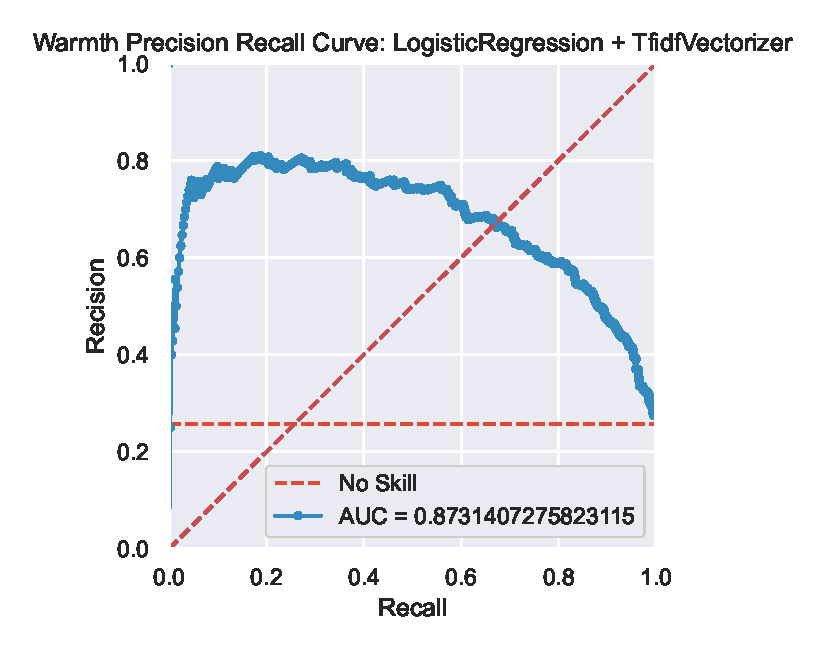
\includegraphics[width=0.75\textwidth]{FT/Figure8.eps}
    \end{center}
    \caption{\textit{Classifying warmth-related framing: Precision-Recall curve for Logistic Regression Classifier with TF-IDF Vectorizer.}}
    \label{figure8}
    \end{figure*}

\begin{figure*}[ht]
    \setlength{\fboxsep}{0pt}%
    \setlength{\fboxrule}{0pt}%
    \begin{center}
    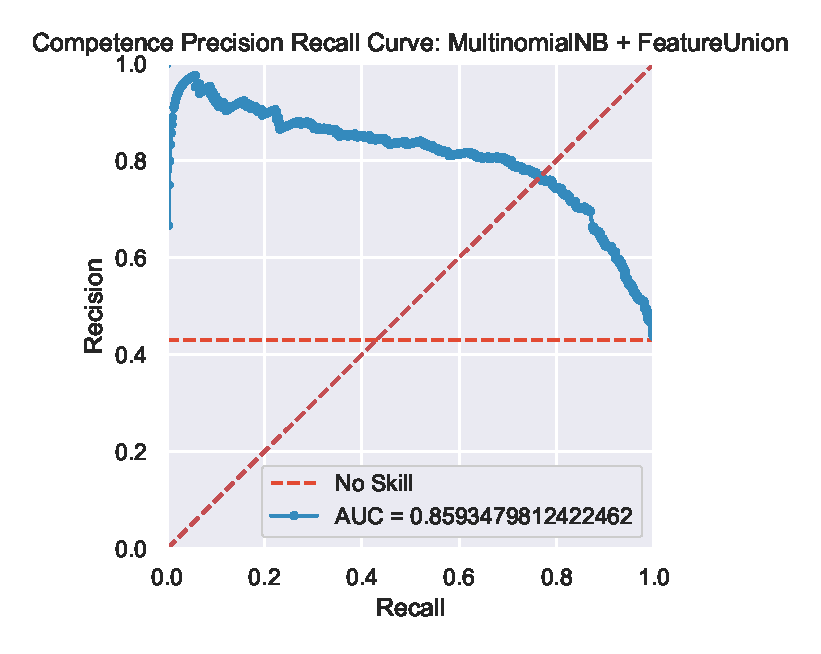
\includegraphics[width=0.75\textwidth]{FT/Figure9.eps}
    \end{center}
    \caption{\textit{Classifying competence-related framing: Precision-Recall curve for Multinomial Naive Bayes (NB) with Feature Union Vectorizer.}}
    \label{figure9}
    \end{figure*}

\begin{figure*}[ht]
    \setlength{\fboxsep}{0pt}%
    \setlength{\fboxrule}{0pt}%
    \begin{center}
    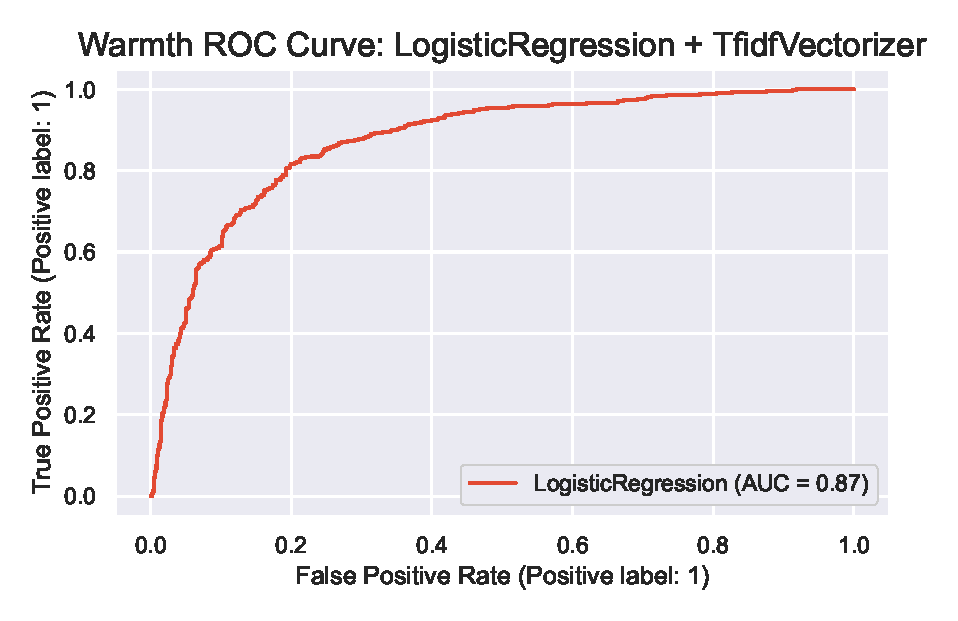
\includegraphics[width=0.95\textwidth]{FT/Figure10.eps}
    \end{center}
    \caption{\textit{Classifying warmth-related framing: ROC curve for Logistic Regression Classifier with TF-IDF Vectorizer.}}
    \label{figure10}
    \end{figure*}

\begin{figure*}[ht]
    \setlength{\fboxsep}{0pt}%
    \setlength{\fboxrule}{0pt}%
    \begin{center}
    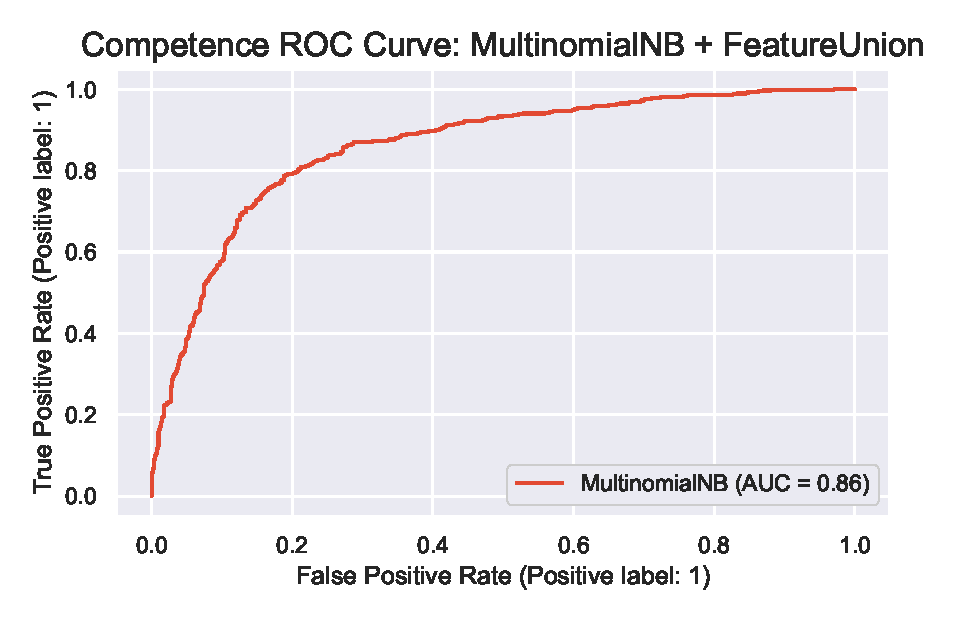
\includegraphics[width=0.95\textwidth]{FT/Figure11.eps}
    \end{center}
    \caption{\textit{Classifying competence-related framing: ROC curve for Multinomial Naive Bayes (NB) with Feature Union Vectorizer.}}
    \label{figure11}
    \end{figure*}

\begin{table}[ht]
    \small\sf\centering
    \caption{\textit{List of words related to warmth and competence obtained from inductive frame analysis}}
    \label{table12}
    \vskip 4pt
    \resizebox{\linewidth-4cm}{!}{%
    \begin{tabular}[]{@{}cc@{}}
    \toprule
    Competence & Warmth\\
    \midrule
    Develop & Supportive\\
    Solution & Collaborative\\
    Strategy & People\\
    Challenge & \makecell[c]{Need (as it relates to meeting other\\people's needs/ aware of others’ needs)}\\
    Product & Community\\
    Persistent & Honest\\
    Assertive & Sympathetic\\
    Ambitious & Friendly\\
    Industrious & Caring\\
    Able & Patient\\
    Capable & Fair\\
    Strong-minded & Helpful\\
    Determined & Polite\\
    Clever & Gentle\\
    Self-reliant & Cooperative\\
    Consistent & Loyal\\
    Competent & Moral\\
    Talented & Warm-hearted\\
    \bottomrule
    \end{tabular}
    }
    \end{table}

\clearpage
\newpage
\section{Appendix B\label{appendix_b}}

\section{Codebook for Bias in Candidate Sourcing Communication Project\label{codebook}}
This study aims to look at the framing of job advertisements from different occupational sectors in the Dutch labor market. Particularly, we examine whether the framing of job advertisements conveys certain characteristics in relation to the company, the offered position, or the ideal prospective candidate. Two main characteristics we are interested in are warmth and competence, and the present codebook focuses on whether job descriptions emphasize warmth or competence related characteristics and traits. Explanations and example-sentences of warmth- and competence-related terms are provided below, under C2.1 and C2.2 respectively.
As coder, you will receive a text file containing job advertisement texts along with a Job ID associated with each. You will then be asked to fill in the coding form based on the text of \uline{each sentence}. We advise the text be kept in view while coding sentences.
\uline{Make special note of the lists of words attached to the end of this codebook titled “Table 12”.} These words can help you identify the terms in a sentence that may convey warmth and/or competence. Although the tables can be helpful, please use your discretion as well in determining the right coding.

\subsection{Description of units of analysis\label{description_of_units_of_analysis}}
Here you can find some guidelines on how to identify each of the units.

\noindent\textbf{Registration Unit:} The registration unit is \uline{every sentence}. This means that you will fill out the coding form once for each sentence you view.
\begin{itemize}
    \item If a bullet-point format is used, and each bullet-point consists of one word, one term, or one sentence, each bullet-point serves as the registration unit. If each bullet-point consists of more than one term (e.g., good communicator, fast learner, skilled programmer) or one sentence, then each term and/or sentence serves as the registration unit.
    \item Headings and subheadings are also coded in a similar manner as single sentences unless they consist of more than one sentence, in which case, each sentence is taken as a single registration unit.
    \item If a sentence contains parentheses, code the portion within the brackets depending on whether it can be a stand-alone sentence. If it is a stand-alone sentence, rules for coding a single sentence apply. If that is not the case, code the parenthesized portion as part of the sentence containing it.
    \end{itemize}

\noindent\textbf{Contextual Unit:} In case you need to clarify the coding of a sentence, consult the sentences immediately before and after it.

\begin{enumerate}[label=\textbf{C\arabic*.}, wide=0pt, itemindent=0.25\textwidth]
    \item \textbf{ADMINISTRATIVE VARIABLES\label{administrative_variables}}
    \begin{enumerate}[label=\textbf{C\arabic{enumi}.\arabic*.}, wide=0pt]
        \item \noindent\textbf{Coder ID}

        This variable is for your personal Coder ID.

        {\small Please write down the coder ID \uline{exactly as is}.}

        \item \noindent\textbf{Job ID}

        This variable is for the Job ID (provided in the text file) that corresponds to the sentence you are coding.

        {\small Please write down the job ID \uline{exactly as is}.}

        \item \noindent\textbf{Sentence}

        This variable contains the sentence to be coded.

        {\small Please paste the sentence from the provided text file.}
        \end{enumerate}

    \item \textbf{SENTENCE-LEVEL VARIABLES\label{sentence_level_variables}}

    \textbf{INSTRUCTIONS FOR CODING\label{instructions_for_coding}}
    \begin{itemize}
        \item Code headings, sub-headings, and bullet-points.
        \item Code parenthesized portions of a sentence separately from the sentence containing it only if the portion within the brackets is a stand-alone sentence.
        \item \uline{A sentence can be coded as containing both warmth AND competence.}
        \item \uline{A sentence can be coded as containing neither warmth NOR competence.}
        \item Try to think critically about the sentence text, i.e., what is being said about the characteristics of company and position, or candidate traits, and how much emphasis is placed on those characteristics.
        \item Pay special attention to the context of a sentence and defer to the contextual units if in doubt.
        \item Table 1 and Table 2 below can be consulted to determine the coding of a sentence but please strongly defer to the contextual units as well as to your own understanding of the sentence.
        \end{itemize}

        \noindent Below are examples of how to code sentences, bullet-points, and sentences with parentheses:

    \noindent\textbf{\small Example: Sentences}

    \noindent\textit{\small “The candidate must be skilled in programming and able to work in a team”.}

    \begin{adjustwidth}{0.75cm}{}
        {\small The above example is considered a single sentence. You must code once for “The candidate must be skilled in coding and able to work in a team”. The coding form is thus filled out one time for this example.}
        \end{adjustwidth}

    \noindent\textbf{\small Example: Bullet-points}

    \noindent\textit{\small “The candidate must be:
    \begin{itemize}
        \item Skilled in programming
        \item Able to work in a team
        \item A fast-learner”
        \end{itemize}}

    \begin{adjustwidth}{0.75cm}{}
        {\small In the above example, the introductory phrase and the three individual bullet-points are each considered a single sentence. You must code once for “The candidate must be”, once for “skilled in coding”, once for “able to work in a team”, and once for “fast-learner”. The coding form is thus filled out four times for this example.}
        \end{adjustwidth}

    \noindent\textbf{\small Example: Sentence with parentheses}

    \noindent\textit{\small “Ensure quality of solution (in line with requirements set)”}

    \centerline{\textbf{VS.}}

    \noindent\textit{\small “Manage project resources (Lead the project team)”}

    \begin{adjustwidth}{0.75cm}{}
        {\small In the first example above, “in line with requirements set” supplements the quality assurance task. It would be difficult to understand what the candidate is required to do without taking the portion before the parentheses into account.You would code this example as one sentence.

        In the second example above, “Lead the project team” is easily understood from a requirements perspective without deferring to the portion before it. Something to keep in mind in the capitalization of the portion within brackets. In the second example, capitalization indicates the independence of the bracketed portion from the part preceding it. You would code this sentence twice, as two separate sentences.}
        \end{adjustwidth}
    \begin{enumerate}[label=\textbf{C\arabic{enumi}.\arabic*.}, wide=0pt]
        \item \noindent\textbf{Sentence warmth assessment}

        This variable indicates whether a sentence is related to \uline{warmth}.

        \noindent\textbf{Definition of warmth and warmth-related skills:}

        \textit{Warmth is characterized by a concern for and understanding of others, supportiveness, helpfulness, sincerity, interpersonal sensitivity, and \uline{people-orientation}. A good indicator of whether a sentence relates to warmth is if elements in the sentence address interpersonal and community-building factors, e.g., dependability, flexibility, and managing team communication.}

        \noindent\textbf{\uline{Remember, a sentence can be coded as both related to warmth AND competence as well as related to neither warmth NOR competence.}}

        \noindent Below are examples of how to code for the presence of warmth in a sentence:

        \noindent\textit{\textbf{Special note:} When terms like international, global, multicultural, etc. are used, focus on whether it relates to teams and people or actual company presence, development, geographic regions, and conglomeratization. The first case relates to warmth whereas the second relates to competence.}

        \noindent\textbf{\small Example: Warmth}

        \noindent\textit{\small “A successful candidate will have a holistic perspective and will be able to adapt the environment to fit the person”.}

        \begin{adjustwidth}{0.75cm}{}
            {\small The above example sentence focuses on adaptation and fitting in an environment. These are interpersonal skills and are related to warmth traits. The coding should reflect that warmth relating traits are present.}
            \end{adjustwidth}

        \noindent\textbf{\small Example: Warmth}

        \noindent\textit{\small “The candidate will develop and manage customers as well as ensure a planned approach to Customer Relationship Management in terms of identifying and strengthening revenue, relationship building and ensuring customer retention and customer visits”.}

        \begin{adjustwidth}{0.75cm}{}
            {\small Although the above example sentence mentions a specific managerial approach, its focus is on skills that are related to customer interactions, e.g., relationship building. This sentence can thus be coded as relating to warmth traits. The coding should reflect that warmth relating traits are present. Note that sentences can also be coded to reflect the presence of competence related traits if applicable.}
            \end{adjustwidth}

        \noindent\textbf{\large \uline{The sentence is:}}

        \noindent {\large 0 = Not related to warmth}

        \noindent {\large 1 = Related to warmth}\\

        \item \noindent\textbf{Sentence competence assessment}

        This variable indicates whether a sentence is related to \uline{competence}.

        \noindent\textbf{Definition of competence and competence-related skills:}

        \textit{Competence is characterized by self-assertion, leadership, analytical and strategic thinking, efficiency, competitiveness, independence, and \uline{task- and outcome-orientation}. A good indicator of whether a sentence relates to competence is if elements in the sentence address technical and productivity-centric factors, e.g., technological skills and managing team outcomes.}

        \noindent\textbf{\uline{Remember, a sentence can be coded as both related to warmth AND competence as well as related to neither warmth NOR competence.}}

        \noindent Below are examples of how to code for the presence of competence in a sentence:

        \noindent\textit{\textbf{Special note:} When terms like international, global, multicultural, etc. are used, focus on whether it relates to teams and people or actual company presence, development, geographic regions, and conglomeratization. The first case relates to warmth whereas the second relates to competence.}

        \noindent\textbf{\small Example: Competence}

        \noindent\textit{\small “This role is responsible for leveraging digital channels to drive traffic and sales to both to our broad network of labs and online via our new eCommerce initiatives”.}

        \begin{adjustwidth}{0.75cm}{}
            {\small The above example sentence focuses on technical skills that are related to competence, e.g., expertise in eCommerce. The coding should reflect that competence related traits are present.}
            \end{adjustwidth}

        \noindent\textbf{\small Example: Competence}

        \noindent\textit{\small “Candidate must have a degree in teaching the English language and be familiar with bilingual education and various international exam programmes like IB and Cambridge”.}

        \begin{adjustwidth}{0.75cm}{}
            {\small Although the above example sentence addresses language and communication, which is an interpersonal skill, the focus of the tasks is on technical and strategic skills, which are related to competence characteristics. The coding should reflect that competence related traits are present.}
            \end{adjustwidth}

        \noindent\textbf{\large \uline{The sentence is:}}

        \noindent {\large 0 = Not related to competence}

        \noindent {\large 1 = Related to competence}\\

        \item \noindent\textbf{Coder Remark}

        This variable is for anything noted by the coder regarding the item.

        {\small Please leave blank if not applicable.}

        \end{enumerate}
    \end{enumerate}

\end{document}
